\documentclass{./../../Latex/notes}

\numberwithin{section}{chapter} 
\numberwithin{subsection}{section} 

\makeatletter
\def\@makechapterhead#1{%
  \vspace*{50\p@}%
  {\parindent \z@ \raggedright \normalfont
    \interlinepenalty\@M
    \Huge \bfseries \phantom{#1} \par\nobreak
    \vskip 40\p@
  }}
\makeatother
\usepackage[colorlinks=true, linkcolor=blue]{hyperref}
\setcounter{tocdepth}{1}

\begin{document}

\title{Lecture Notes \\ Econ 340: Economic Research Methods}
\author{Div Bhagia}
\date{}

\begin{titlepage}
    \maketitle
    \tableofcontents    
\end{titlepage}

\chapter{Summation Notation}
\vspace{-6cm} 
\documentclass{./../../Latex/handout}
\begin{document}
\thispagestyle{plain}
\newcommand{\mytitle}{Summation Notation}
\myheader{\mytitle}

The capital sigma ($\Sigma$) stands for summing everything on the right. 
$$ \sum_{i=1}^N X_i = X_1 + X_2 + ... + X_N $$
When we have sets, the index $i$ denotes the $i$-th position in the set. 

\textit{Example}: For $X = \{1, 3, 5, 1\}$, we have $\sum_{i=1}^3 X_i = X_1 + X_2 + X_3 = 1 + 3 + 5 = 9$

\textit{Note}: Another way of using a summation sign is to write $\sum_{x \in A} x $, which refers to summing up all elements in $A$. Similarly, to sum up $x$ for all possible values $x$, we can simply write $\sum_x x$. \\


\underline{Things you CAN do to summations:}
\begin{enumerate}
\item Pull constants out of them or into them.
$$ \sum_{i=1}^N b X_i = b \sum_{i=1}^N X_i  $$ \\
\textit{Example}: $ \sum_{i=1}^2 b X_i = b X_1 + b X_2 = b(X_1 + X_2) = b \sum_{i=1}^2 X_i $ \\
\item Split apart (or combine) sums (addition) or differences (subtraction)
$$ \sum_{i=1}^N (b X_i + c Y_i) = b \sum_{i=1}^N X_i  + c \sum_{i=1}^N Y_i $$ \\
\textit{Example}: $\sum_{i=1}^2 (X_i - 2 Y_i) = (X_1-2 Y_1) + (X_2-2 Y_2) = X_1 + X_2 - 2(Y_1 + Y_2)$. So we can write $$\sum_{i=1}^2 (X_i - 2 Y_i) = \sum_{i=1}^2 X_i - 2 \sum_{i=1}^2 Y_i $$ \\
\item Multiply through constants by the number of terms in the summation
$$ \sum_{i=1}^N (a+b X_i)= aN + b \sum_{i=1}^N X_i  $$ \\
\textit{Example}: $\sum_{i=1}^3 a = a + a + a = 3a $. \\
\end{enumerate}

\underline{Things you CAN NOT do to summations:}
\begin{enumerate}
\item Split apart (or combine) products (multiplication) or quotients (division).
$$ \sum_{i=1}^N X_i Y_i \neq  \sum_{i=1}^N X_i \times \sum_{i=1}^N Y_i   $$
\textit{Example}: Note that $\sum_{i=2}^N X_i Y_i = X_1 Y_1 + X_2 Y_2 $, while $(\sum_{i=1}^2 X_i) \cdot (\sum_{i=1}^2 Y_i) = (X_1+X_2)(Y_1 + Y_2) = X_1 Y_1 + X_2 Y_2 + X_1 Y_2 + X_2 Y_1 $. \\

\item Move the exponent out of or into the summation.
$$ \sum_{i=1}^N X_i^a \neq  \left(\sum_{i=1}^N X_i\right)^a $$
\textit{Example}: Note that $\sum_{i=1}^2 X_i^2 =  X_1^2 + X_2 ^2$, while  $\left(\sum_{i=1}^2 X_i\right)^2 = (X_1 + X_2)^2 = X_1^2 + X_2 ^2 + 2X_1 X_2$. \\
\end{enumerate}



\end{document}

\chapter{Describing Data}
\vspace{-6cm}
\documentclass{./../../Latex/handout}
\begin{document}
\thispagestyle{plain}
\myheader{Describing Data}

\vspace{-1cm}
\section{What is a variable?}

A \textit{variable} is multiple observations of the same measurement. Variables may be classified into two main categories: continuous and categorical (or discrete).
\begin{itemize}
\item \textit{Continuous}: can take any value in an interval (e.g., income, age, GPA, rent, etc.)
\item \textit{Categorical (or discrete)}: assigns observations in different groups  (e.g., gender, race, religious affiliation, educational attainment, etc.)
\end{itemize}
A categorical variable with two categories is called a \textit{binary} variable. 

Many questions in economics and other social sciences are concerned with cause-and-effect relationships. When studying such questions, we refer to the cause as the \textit{independent} variable. The \textit{dependent} variable is the effect. Its value depends on changes in the independent variable. Finally, a \textit{control} variable is a variable that might affect \underline{both} the \textit{dependent} and the \textit{independent} variables, and we might want to account for it while studying our causal relationship of interest. 
\begin{center}
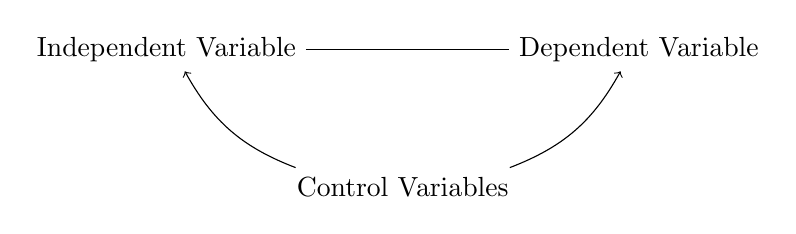
\begin{tikzpicture}
\node (1) at (0,0) {Control Variables};
\node (2) at (-3,1.75) {Independent Variable};
\node (3) at (3,1.75) {Dependent Variable};
\path (2) edge  (3);
\path[->] (1) edge[bend left=20] (2);
\path[->] (1) edge[bend right=20] (3);
\end{tikzpicture}	
\end{center}

The dependent variable is also called the \textit{outcome} or \textit{response} variable. In contrast, the independent variable is also called the \textit{predictor} or \textit{explanatory} variable. We will also refer to \textit{control} variables as \textit{confounding} variables. 

\section{Empirical Distribution of a Variable}

A useful way to learn about a variable is by looking at how often different values of this variable occur. This information is summarized by a variable's empirical \textit{distribution}. We can look at the proportion of observations in each category for categorical variables. In particular, we can calculate the \textit{relative frequency} as follows:

$$ \text{Relative frequency} =  \frac{\text{Number of observations in a category}}{\text{Total number of observations}} $$ 

 If $n$ denotes the total number of observations and $n_k$ denotes the number of observations that fall in category $k$, then we can calculate the relative frequency $f_k$ as follows:
$$ f_k = \frac{n_k}{n} $$

The relative frequency $f_k$ tells us the proportion of observations in category $k$. 

The following is an example of a \textit{frequency distribution table} for the outcome from 100 die rolls. 

\begin{center}
\begin{tabular}{cccc}
\toprule
Outcome & Count & Proportion & Cumulative \\
\midrule
1 &  18 & 0.18 & 0.18 \\
2 & 18 & 0.18 & 0.36 \\
3 & 12 & 0.12 & 0.48 \\
4 & 16 & 0.16 & 0.64 \\
5 & 21 & 0.21 & 0.85 \\
6 & 15 & 0.15 & 1 \\
\hline
Total & 100 & 1 & \\
\bottomrule
\end{tabular} 
\end{center}

The cumulative frequency is calculated by adding each frequency from a frequency distribution table to the sum of its predecessors. 

Continuous variables can take many different values, so it is not possible to look at how many observations take each possible value. Instead, we can look at how many observations fall in a particular interval. 

The graphical version of the frequency distribution table is a \textit{histogram}. The $x$-axis of a histogram presents the possible outcomes or intervals for the variable, while the $y$-axis presents the number or proportion of outcomes in each group. Below is a histogram of household income. 

\includegraphics{./../../Output/hhi_hist.pdf}

Note that the distribution is skewed to the right due to a small number of outliers with really high incomes. 

\section{Measures of Central Tendency}

While a frequency distribution table or a histogram is a good way to learn about a variable, we only sometimes want to present a long table or a figure. We want a single number that can summarize this variable. A few options:
\begin{itemize}
\item[] \textit{{Mean}}:  the average value
\item[] \textit{{Median}}: the middle value 
\item[] \textit{{Mode}}: the most frequent value
\end{itemize} 

To calculate the median, you find the middle value. If the number of observations is even, you take the average of the two middle values. 

Mean and median are frequently employed in applied work. While the mean suffices for most purposes, it is more sensitive to outliers than the median because it considers all values, not just the middle values. For the distribution of household income above, the mean is \$112,900, and the median is \$91,600. Mean earnings are higher than the median, reflecting that the mean is pushed upwards as it is more affected by the outliers with really high incomes in the data. 

To calculate the mean, you add up all the observations and divide by the number of observations. A sample mean is usually denoted by $\bar{X}$ and can be calculated as:

$$ \bar{X} = \frac {\sum_{i=1}^n X_i}{n} $$ 

Here $n$ is the sample size. 

The population mean is denoted by $\mu$. \\

\fbox{\begin{minipage}{\textwidth}
Some things to note about the mean: 

\begin{itemize}
\item $\sum_{i=1}^n X_i = n \bar{X}$ 
\item Deviations from the mean are always zero
$$ \sum_{i=1}^n (X_i-\bar{X}) =  \sum_{i=1}^n X_i - n \bar{X} = n \bar{X}- n \bar{X}=0 $$
\item We can always write
$$ \bar{X} = \frac {\sum_{i=1}^n X_i}{n} = \frac{1}{n}\sum_{i=1}^n X_i = \sum_{i=1}^n \frac{X_i}{n} $$
\end{itemize}
\end{minipage}} \\ 

\subsection*{Mean from Grouped Data}

If data are grouped, we can use the frequency distribution table to calculate the mean.  In particular, for $K$ groups, we use the following formula: 

$$ \bar{X} = \frac{\sum_{k=1}^K n_k X_k}{n} = \sum_{k=1}^K f_k X_k $$

 Example. Say, we have the following observations on a variable $X$:  $$1,1,3,3,3,4,5$$ One way to find the mean:
 $$ \frac{1+1+3+3+3+4+5}{7} = \frac{20}{7}  $$
 
 Another way to find the mean:
 \begin{center}
\begin{tabular}{|c|c|p{1cm}|p{1cm}|}
\hline
$X_k$ & \hspace{0.5em} $n_k$ & \hspace{0.2em} $f_k$ & $f_k X_k$ \\
\hline
 1 & 2 & 2/7 & 2/7 \\
 \hline
3 &  3 & 3/7 & 9/7 \\
\hline
4 & 1 & 1/7 & 4/7 \\
\hline
5 &  1 & 1/7 & 5/7  \\
\hline
Total & 7 & 1 & 20/7 \\
\hline
\end{tabular}
 \end{center}
 
 Note that both approaches are equivalent, as all we do by using the frequency distribution table is group observations with the same values. 
 \begin{align*}
 	\frac{1+1+3+3+3+4+5}{7} &= \frac{(2\times 1)+(3\times 3)+(1\times 4)+(1 \times 5)}{7} \\
 	&= 2.\frac{1}{7} + 3.\frac{3}{7} + 4.\frac{1}{7}+ 5.\frac{1}{7}
 \end{align*}


\subsection*{Weighted Mean}
The \textit{weighted mean} of a set of data is given by:

$$ \bar{X} = \frac{\sum_{i=1}^n\omega_i X_i}{\sum_{i=1}^n \omega_i} $$

where $\omega_i$ is the weight of the $i^{th}$ observation. When weights sum up to 1 (i.e. \(\sum_{i=1}^n \omega_i=1\)) we can simply write the weighted mean as:

$$ \bar{X} = \sum_{i=1}^n\omega_i X_i$$ 

When we calculate the unweighted mean, we put equal weight on all observations in the data. However, sometimes we want to put a higher weight on some observations than others; in such cases, we use the weighted mean. 


\section{Percentiles}
The \textit{$P^{th}$ percentile} is a value such that $P$\% of observations are at or below that number. \\~\\
The 50th percentile is called the median. The 25th and 75th percentiles are called the 1st and 3rd quartiles, respectively.

\section{Measures of Variance}

Measures of central tendency tell us about the average observation in the data. However, it doesn't say anything about this variable's dispersion or variation. One way to learn about dispersion would be to look at the minimum and maximum values a variable takes. This is called the \textit{range} of the variable. Another way is to look at how far observations are away from the mean, so calculate the variance as follows. \\

\textit{Population Variance}
$$ \sigma_X^2 = \frac{1}{N} \sum_{i=1}^N (X_i-\mu_X)^2 $$
\textit{Sample Variance}
$$ S_X^2 = \frac{1}{n-1} \sum_{i=1}^n (X_i-\bar{X})^2 $$

If there is more dispersion in the data, the variance will be higher. This is because we calculate the mean by taking the average of square deviations from the mean. If many observations are further below or above the mean, the sum of square deviations will be larger. 

For the sample variance, the denominator is $n-1$ instead of $n$. This is because observations in the sample are closer to the sample mean than the population mean. The variance estimator uses the sample mean and hence underestimates the actual variance of the population. Dividing by $n-1$ instead of $n$ corrects for that bias. 

However, it isn't easy to interpret the variance since it is in \textit{squared units}. So we often convert the variance back to its original units by taking the square root of it. This quantity is called the standard deviation. 


\textit{Standard Deviation}
$$ \sigma_X = \sqrt{\sigma_X^2} \quad \quad S_X = \sqrt{S_X^2} $$ \\

\textit{Example.}
\begin{center}
	\begin{tabular}{|c|c|c|}
  \hline
  $X_i$ & $X_i-\mu$ & $(X_i-\mu)^2$ \\
  \hline
  2 & -3 & 9 \\
  \hline
  5 & 0 & 0 \\
  \hline
  8 & 3 & 9 \\
  \hline
  Total & 0 & 18 \\
  \hline
  \end{tabular}
\end{center}

We can calculate the variance as follows: 
$$ \sigma_X^2 = \frac{1}{3} \sum_{i=1}^3 (X_i-\mu_X)^2 = \frac{18}{3} = 6$$
The standard deviation is $\sigma_X = 2.45$. 

Note that we can use the frequency distribution table for grouped data to calculate the variance. In which case, 
$$ \sigma_X^2 = \sum_{k=1}^K f_k (X_k-\mu_X)^2 $$

 For the sample variance, we will need to do the $n-1$ correction as follows:
 $$ S_X^2 = \frac{n}{n-1} \sum_{k=1}^K f_k (X_k-\bar{X})^2 $$


\section{Z-Score}

Z-score is defined as:
$$ Z = \frac{X - \mu}{\sigma} $$
Z-score tells us how many standard deviations any particular observation is away from the mean.

Example. Say we have two hypothetical countries Mushroom Kingdom (MK) and Bowser's Kingdom (BK). Now say $$ \mu_{MK} = 50,000 \quad \quad  \mu_{BK} = 50,000 $$
$$ \sigma_{MK} = 3,000 \quad \quad  \sigma_{BK} = 5,000 $$

Someone earning \$ 45,000 in MK is $5000/ 3000 =1.66$ standard deviations below the mean. While someone earning \$ 45,000 in BK is $5000/ 5000 =1$ below the mean. Why the difference? Z-score standardizes both distributions and tells us how many people are between the person who earns 50K and 45K. 

\section{Correlation and Covariance}

While so far, we have been talking about describing one variable. Most often, we are interested in the relationship between two different variables. For instance, we might be interested in whether cars with better fuel economy have lower horsepower. To learn about such relationships, we can calculate the \textit{covariance}:

$$ \sigma_{XY} = \frac{1}{N}\sum_{i=1}^N (X_i-\mu_X)(Y_i-\mu_Y) \quad (Population) $$
$$ S_{XY} = \frac{1}{n-1}\sum_{i=1}^n (X_i-\bar{X})(Y_i-\bar{Y}) \quad (Sample) $$

Covariance indicates whether there is a positive or negative relationship between two variables. 

Why does this formula work? If it is, in fact, true that there is a negative relationship between fuel economy as measured by MPG and horsepower. Then for many observations in our data, $(X_i-\mu_X)(Y_i-\mu_Y)$ will be negative. $(X_i-\mu_X)(Y_i-\mu_Y)$ is negative every time $X_i$ is above its mean but $Y_i$ is below its mean or vice versa. 

Similarly, $(X_i-\mu_X)(Y_i-\mu_Y)$ is positive for any observation if both $X_i$ and $Y_i$ are above the mean. The covariance is positive if $(X_i-\mu_X)(Y_i-\mu_Y)$ is positive on average. If there is no clear relationship between the two variables, for some observations, $(X_i-\mu_X)(Y_i-\mu_Y)$ will be negative, while for some, it will be positive, leading the covariance to go towards 0. 

In other words, if two variables tend to be above average at the same time or below average at the same time, then we add a positive number to the numerator for the covariance for most observations, increasing the covariance. If they have nothing to do with each other, we add a positive number sometimes and a negative number other times, canceling each other and giving us a covariance of 0. 

The upper and lower limits for the covariance depend on the variances of the variables involved. These variances, in turn, can vary with the scaling of the variables, so even a change in the units of measurement can change the covariance. Thus, covariance is only helpful in finding the direction of the relationship between two variables and not the magnitude. 

We can obtain the \textit{correlation coefficient} of two variables by dividing the covariance of these variables by the product of the standard deviations of both variables. Correlation also indicates the strength of the relationship in addition to the direction.
$$ \rho_{XY} = \frac{ \sigma_{XY}}{\sigma_X \sigma_Y}  \quad (Population) $$
$$ r_{XY} = \frac{ S_{XY}}{S_X S_Y} \quad (Sample) $$

\fbox{\begin{minipage}{\textwidth}
Things to note about the correlation coefficient:
\begin{itemize}
\item Measures the strength and direction of the linear relationship between two variables
\item Bounded between $-1$ and $1$
\item If $\rho=0$, there is no linear relationship between the two variables. If $\rho=1$ or $\rho=-1$, there is a perfect linear relationship.
\item If $\rho>0$, then when $X$ is above (below) $\bar{X}$, $Y$ is above (below) $\bar{Y}$.
\item If $\rho<0$, then when $X$ is above (below) $\bar{X}$, $Y$ is below (above) $\bar{Y}$. 
\end{itemize}
\end{minipage}}
\vspace{1em}

Finally, correlation is not causation! Particularly for two reasons:
\begin{itemize}
\item[1.] Reverse causality: A high correlation between education and household income could come from either ``more education $\rightarrow$ higher household income'' or ``higher household income $\rightarrow$ more education.''
\item[2.] Other factors: It could be another factor like generational wealth is correlated with \underline{both} the likelihood of getting more education and having a higher household income. 
	
\end{itemize}


\end{document}

\chapter{Random Variables}
\vspace{-6cm}
\documentclass{./../../Latex/handout}

\begin{document}
\thispagestyle{plain}
\myheader{Random Variables}

\vspace{-1cm}
\section{Single Random Variable}

A random variable is a variable that takes different values under different scenarios. The likelihood of these different scenarios is summarized by the distribution of the random variable. We will denote a random variable by $X$ and realizations of it by $x$. 

Random variables can either be discrete or continuous. A \textit{discrete} random variable has a countable number of possible values. While \textit{continuous} random variables can take any value in a given interval. 

%%%%% Discrete Random Variables
\subsection{Discrete Random Variables}

The \textit{probability distribution function} (PDF) for a discrete random variable $X$ is given by:
$$ f(x) = Pr(X=x) $$
where $0 \leq f(x) \leq 1$ for all $x$ and $\sum_x f(x) = 1$. 

The \textit{cumulative distribution function} (CDF) for a discrete random variable $X$ is given by: 
$$ F(x_0) = Pr(X \leq x_0) = \sum_{x \leq x_0} f(x) $$ 
\textit{Example.} $X$ is the outcome of rolling a die. \vspace{-0.4cm}
% Table: Die Roll 
\begin{center}
\begin{tabularx}{0.5\textwidth}{XXX}
\toprule
$x$ & $f(x)$ & $F(x)$ \\ 
\midrule
1 & 1/6 & 1/6 \\
2 & 1/6 & 2/6 \\
3 & 1/6 & 3/6 \\
4 & 1/6 & 4/6 \\
5 & 1/6 & 5/6 \\
6 & 1/6 & 1 \\
\bottomrule
\end{tabularx}
\end{center}

% Figure: Die Roll
\begin{figure}[!h]
\caption{Outcome from a Die Roll}
\centering
\begin{tabular}{cc}
\subfloat[Probability Distribution Function]{\includegraphics{./../../output/die_roll_pdf.pdf}} & 
\subfloat[Cumulative Distribution Function]{\includegraphics{./../../output/die_roll_cdf.pdf}} 
\end{tabular}
\end{figure}

\textit{Bernoulli Random Variable} is a special type of discrete random variable that only takes two values 1 and 0. It is also called a \textit{binary} variable. 

$$ X = \begin{cases} 
 	1 \quad \text{with probability $p$} \\
 	0 \quad \text{with probability $1-p$} 
 \end{cases}
$$


%%%%% Continuous Random Variables
\subsection{Continuous Random Variables}

Because of continuum of possible values, it is not feasible to list the probability of each possible value of a continuous random variable. So we instead have the \textit{probability density function} (PDF), denoted by $f(x)$. The area under the curve $f(x)$ gives us the probability of $X$ falling in certain intervals. The \textit{probability density function} is defined as:

$$ Pr(a \leq x \leq b) =  \int_{a}^{b} f(x) \partial x $$

where $f(x)>0$ for all $x$ and $\int_{-\infty}^{\infty} f(x) \partial x =1 $. 

Note that for continuous random variables, $Pr(X=x)=0$. This is just to say that it is very very unlikely that any particular value will be realized because there are infinite possibilities. 

The integral $\int^{b}_{a}$ is the continuous analog of the sum. You don't need to know how to solve an integral, but remember it is like taking a sum over continuous values. The limits of the integral, $a$ and $b$, define the interval over which we are taking this sum.

The \textit{cumulative density function} (CDF) for a continuous random variable $X$ is given by: 

$$ F(x_0) = Pr(X \leq x_0) = \int_{-\infty}^{x_0} f(x) \partial x$$

Note that, $ Pr(a \leq x \leq b) = F(b) - F(a) $. 

\textit{Example.} Let's say the distribution for the height of individuals in the world is given by the following probability density function: 

\begin{figure}[!h]
\centering
\includegraphics{./../../output/height_norm_pdf.pdf} \\
\end{figure}

We need to find the corresponding area under the curve to find the probability of height being in particular intervals. 

\begin{figure}[!h]
\begin{tabular}{cc}
\subfloat[$Pr(150<X<175)$]{\includegraphics{./../../output/height_norm2_ho.pdf}} &
\subfloat[$Pr(X<150)$]{\includegraphics{./../../output/height_norm2_ho2.pdf}} 
\end{tabular}
\end{figure}

The CDF corresponding to the above PDF looks like:

\begin{figure}[!h]
\centering
\includegraphics{./../../output/height_norm_cdf.pdf} 
\end{figure}

%%%%% Expectation and Variance
\subsection{Expectation and Variance of Random Variables}

The \textit{expectation} or \textit{expected value} or the \textit{mean} of a random variable gives us the average value of this variable over many repeated trials or occurrences. We can compute the expectation as a weighted average of possible outcomes, where the weights are probabilities.  

The expectation of a discrete random variable is given by:

$$ \mu_X = E(X) = \sum_x x f(x) $$

The expected value for a continuous random variable is given by:
$$ \mu_X = E(X) = \int_x x f(x) \partial x $$

The \textit{variance} measures the dispersion or the ``spread'' of a
probability distribution. The variance for a random variable is given by:

$$\sigma_X^2 = Var(X) = E [(X-\mu_X)^2]   $$ 

In other words, variance is the expected value of the square of deviations of $X$ from its mean. 

Using the definition of expectation for a discrete random variable, we can write:
$$\sigma_X^2 = Var(X) = E [(X-\mu_X)^2] = \sum_x (x-\mu_X)^2 f(x)  $$ 

Alternative formula for the variance:  $Var(X) = E[(X-\mu_X)^2] = E(X^2)-\mu_X^2$.

Variance is in units of the square of $X$. Therefore we use \textit{standard deviation}, which is the square-root of variance:
$$\sigma_X = \sqrt{\sigma_X^2}$$ 


\textit{Example}. We can calculate the expected value and variance for the outcome of rolling a die as follows:
\begin{center}
\begin{tabularx}{0.75\textwidth}{XXXX}
\toprule
$x$ & $f(x)$ & $xf(x)$ & $(x-\mu_X)^2 f(x)$ \\ 
\midrule
1 & 1/6 & 1/6 & (-2.5)$^2$/6 \\
2 & 1/6 & 2/6 & (-1.5)$^2$/6 \\
3 & 1/6 & 3/6 & (-0.5)$^2$/6 \\
4 & 1/6 & 4/6 & (0.5)$^2$/6 \\
5 & 1/6 & 5/6 & (1.5)$^2$/6 \\
6 & 1/6 & 6/6 & (2.5)$^2$/6 \\ \midrule
Total & - & 21/6 & 17.5/6 \\
\bottomrule
\end{tabularx}
\end{center}
$$ \mu_X = E(X) = \sum_{x} xf(x) = \frac{21}{6} = 3.5 $$ 
$$ Var(X) = \sum_x (x-\mu_X)^2 f(x) = \frac{17.5}{6} $$ 

\textit{Example}. The expected value and variance for a binary random variable that takes value 1 with probability $p$ and 0 with probability $1-p$ is given by:
$$ \mu_X = E(X) =  \sum_{x} xf(x) = 1.p + 0.(1-p) = p$$
$$ Var(X) =  \sum_{x} (x-\mu_X)^2 f(x) = (1-p)^2.p + (0-p)^2.(1-p) = p(1-p)$$
Using the alternative formula for variance:
$$ Var(X) = E(X^2)-\mu_X^2 = 1^2.p +0^2.(1-p) -\mu_X^2 = p-p^2 = p(1-p)$$

\section{Normal and Standard Normal Distribution} 

\subsection{Normal Distribution}
There are lots and lots of probability distributions that are used for modeling different variables. For example, \textit{uniform} distribution is a distribution with constant probability. There are many more, Bernoulli, binomial, gamma, beta, Poisson, and so on. 

 However, one distribution that appears over and over again is the \textit{normal distribution}. The distribution of a lot of things like height, birthweight, IQ, etc. is normal. The normal distribution is symmetric (i.e., the left and right tails are the same sizes and there’s no skew). For this reason, sometimes it is informally referred to as a bell curve. We express normal distribution with mean $\mu$ and variance $\sigma^2$ as follows:
 $$ N(\mu, \sigma^2) $$
  
Figure 2 presents normal distributions with different means and variances.  \\
 \begin{figure}[!h]\caption{Normal distributions with different means and variances}
\centering
\begin{tabular}{c}
\subfloat{\includegraphics[scale=0.85]{./../../output/norm1}} \\
\subfloat{\includegraphics[scale=0.85]{./../../output/norm2.pdf}} \\
\end{tabular}
\end{figure}

The distribution of height that we saw in the above example was a normal distribution with a mean of 169 and a variance of 225. In which case, we can write $height \sim N(169, 225)$, which is short-form for saying height is normally distributed with mean 169 and variance 225. 

\subsection{Standard Normal Distribution}
The normal distribution with mean 0 and variance 1 is called the \textit{standard normal distribution} and is denoted by $N(0,1)$. Random variables that have a $N(0,1)$ distribution are often denoted by $Z$. 

In fact, we can standardize any normally distributed variable into a standard normal variable by subtracting the mean of the normal variable from each value in the distribution and then dividing by the standard deviation of the distribution. Given $X \sim N(\mu, \sigma^2)$, the standardized random variable is given by:
$$ Z = \frac{X-\mu}{\sigma} $$
Here, $Z \sim N(0,1)$. To see why this is the case, note that when we standardize $X$, we subtract the mean $\mu$ from each value of $X$. This has the effect of shifting the distribution so that its center is at 0. Next, we divide each value by the standard deviation $\sigma$. This has the effect of scaling the distribution so that its spread equals 1.

\subsection{Finding the area under the curve}

We are often interested in finding the probability that a random variable lies in a particular interval. For example, say $X \sim N(3, 16)$, and we want to calculate $Pr(X \geq 5)$. As we said before, to find this probability, we need to calculate the following area under the curve:\\

 \begin{figure}[!h]
 \centering	
\begin{tikzpicture}
\begin{axis}[
  no markers, domain=3-3*4:3+3*4, samples=100,
  axis lines*=left, xlabel=X, ylabel=$f(X)$,
  %every axis y label/.style={at=(current axis.above origin),anchor=south},
  height=4.5cm, width=8cm,
  xtick={-5, -3, -1, 1, 3, 5, 7, 9, 11}, %ytick=\empty,
  enlargelimits=false, clip=false, axis on top,
  ]
  \addplot [very thick,black] {gauss(3, 4)}; 
  \addplot [fill=gray!30, draw=none, domain=5:3+3*4] {gauss(3, 4)} \closedcycle;
%\draw[->, line width=1pt](axis cs: 185, 0.0125)--(axis cs: 205, 0.0125);
%\node at (axis cs: 0, 0.2) { 95\%};
\end{axis}
\end{tikzpicture}
 \end{figure}

However, it can be difficult and time-consuming to calculate the area by hand. Instead, we can standardize this variable and use the \textit{standard normal table} to find this area. The standard normal table provides the area under the standard normal distribution curve for different values of $Z$. 

Given $X \sim N(3, 16)$, 
$$ Z = \frac{X-3}{4} \sim N(0,1) $$

Note that, 
  $$ Pr(X \geq 5) = Pr\left(\frac{X-3}{4} \geq \frac{5-3}{4}\right) = Pr(Z \geq 0.5)  $$
 We can now refer to the standard normal table and find that $Pr(Z \geq 0.5)$ equals 0.3085. The figure below presents this probability as the area under the curve standard normal curve. \\

 \begin{figure}[!h]
 \centering	
\begin{tikzpicture}
\begin{axis}[
  no markers, domain=-3:3, samples=100,
  axis lines*=left, xlabel=Z, ylabel=$f(Z)$,
  %every axis y label/.style={at=(current axis.above origin),anchor=south},
  height=4.5cm, width=8cm,
  xtick={-1.96, 0, 0.5, 1.96}, %ytick=\empty,
  enlargelimits=false, clip=false, axis on top,
  ]
  \addplot [very thick,black] {gauss(0, 1)}; 
  \addplot [fill=gray!30, draw=none, domain=0.5:3] {gauss(0, 1)} \closedcycle;
%\draw[->, line width=1pt](axis cs: 185, 0.0125)--(axis cs: 205, 0.0125);
\end{axis}
\end{tikzpicture}
 \end{figure}


\fbox{\begin{minipage}{\textwidth}
Given $X \sim N(\mu, \sigma^2)$, general recipe to find $Pr(x_0<X<x_1)$:
\begin{itemize}
  \item Find $z_0 = (x_0-\mu)/\sigma$ and $z_1 = (x_1-\mu)/\sigma$
  \item Use standard normal table to find $Pr(z_0<Z<z_1)$ 
\end{itemize}

\end{minipage}} \\ 

\textit{Example.} Given $X \sim N(3, 16)$, we want to find $Pr(2<X<5)$. Here $x_0 = 2, x_1=5$, we can find that  $z_0 = (2-3)/4=-0.25$ and $z_1=(5-3)/4=0.5$. Now we just need to look at the standard normal table and find $Pr(-0.25<Z<0.5)$.

Alternatively, sometimes we wish to identify the value of $x$ for which the probability $Pr(X < x)$ or $Pr(X > x)$ equals a specific value $p$. This can be achieved in a similar manner by using the standard normal table. In particular, we need to find the corresponding value $z$ that satisfies $Pr(Z < z)$ or $Pr(Z > z)$, and then transform it back to obtain $x$. 

\fbox{\begin{minipage}{\textwidth}
Given $X \sim N(\mu, \sigma^2)$ and $Pr(X<x)=p$, to find $x$ : 
\begin{itemize}
  \item Use standard normal table to find $z$ where $Pr(Z<z)=p$ 
  \item Find $x = \mu + z \cdot \sigma $  
\end{itemize}
This follows analogously for when we are given $Pr(X>x)=p$.
\end{minipage}} \\ 


\section{Multiple Random Variables}

\subsection{Joint and Marginal Distribution}

The \textit{joint probability distribution} of two discrete random variables $X$ and $Y$, is the probability that the random variables simultaneously take on certain values.
$$ f(x,y) = Pr(X=x, Y=y)  $$
\vspace{0.25em}

\textit{Example}. The table below gives us the probability of possible commute times and rain on a given day. \\~\\
\begin{tabularx}{0.95\textwidth}{cccc}
\toprule
	& Rain $(X=1)$ & No Rain $(X=0)$ & Total \\
	\midrule
60-min commute ($Y=60$) & 0.3  & 0.2 & 0.5 \\ 
30-min commute ($Y=30$) & 0.1 & 0.4 & 0.5 \\
\midrule
 Total & 0.4 & 0.6 & 1 \\
 \bottomrule \\
\end{tabularx}

The \textit{marginal probability distribution} of a random variable $Y$ is just another name for its probability distribution. In particular, 
$$ f(y) = Pr(Y=y) = \sum_{x} Pr(X=x, Y=y) $$

For example, the probability of having a 60-minute commute is given by the sum of probability of having a 60-minute commute and no rain and the probability of having a 60-minute commute and rain. 
$$ Pr(Y=60) = Pr(X=1, Y=60) + Pr(X=0, Y=60) = 0.3 + 0.2 = 0.5 $$


\subsection{Conditional Probability and Bayes Rule}
The distribution of a random variable $Y$ conditional on another random variable $X$ taking on a specific value is called the \textit{conditional
distribution} of $Y$ given $X$.
$$ f(y|x) = Pr(Y=y| X=x) = \frac{Pr(X=x, Y=y)}{Pr(X=x)} = \frac{f(x,y)}{f(x)}  $$

For example, the probability of having a 60-minute commute conditional on rain is given by:
$$ Pr(Y=60| X=1) = \frac{Pr(X=1, Y=60)}{Pr(X=1)}  = \frac{0.3}{0.4} = \frac{3}{4} $$

While the probability of having a 60-minute commute conditional on no rain is given by:
$$ Pr(Y=60| X=0) = \frac{Pr(X=0, Y=60)}{Pr(X=0)}  = \frac{0.2}{0.6} =\frac{1}{3} $$

Remember, the unconditional probability of having a 60-minute commute was given by 0.5.

The \textit{conditional expectation} of $Y$ given $X$ is the mean of the conditional distribution of $Y$ given $X$. \\
$$ E(Y|X=x) = \sum_{y} y Pr(Y=y | X=x) $$

For the example above, 
$$ E(Y|X=1) = 60.Pr(Y=60 | X=1) + 30.Pr(Y=30 | X=1) = 60 \cdot \frac{3}{4} + 30 \cdot \frac{1}{4}  = 52.5 $$
Similarly,
$$ E(Y|X=0) = 60.Pr(Y=60 | X=0) + 30.Pr(Y=30 | X=0) = 60 \cdot \frac{1}{3} + 30 \cdot \frac{2}{3}  = 40 $$
So by comparing $E(Y|X=1)$ and $E(Y|X=0)$, we can find out how rain affects the average commute time. 

\textit{Bayes' rule} says that the conditional probability of $Y$ given $X$ is the conditional probability of $X$ given $Y$ times the relative marginal probabilities of $Y$ and $X$:
$$ Pr(Y=y| X=x) = \frac{Pr(X=x| Y=y)Pr(Y=y)}{Pr(X=x)}   $$

This is a very useful law because it says that we can deduce conditional probabilities from the reverse conditional probability with the help of marginal probabilities. 

\subsection{Law of Iterated Expectations}
The mean of $Y$ is the weighted average of the conditional expectation of $Y$ given $X$, weighted by the probability distribution of $X$.
$$ E(Y) = \sum_x E(Y|X=x) Pr(X=x) $$
More compactly,
$$ E(Y) = E(E(Y|X)) $$
E.g. the mean height of adults is the weighted average of the mean height
of men and women, weighted by their proportions.  

\subsection{Independence and Uncorrelatedness}

Two random variables $X$ and $Y$ are independently distributed, or \textit{independent}, if knowing the value of one of the variables provides no information about the other. That is,
$$ Pr(Y=y | X=x) = Pr(Y=y)  $$
Then by Bayes' rule:
$$ Pr(X=x, Y=y) = Pr(X=x) Pr(Y=y)  $$
\textit{Example}: Two consecutive coin tosses. \\~\\
Note: We can equivalently say that $X$ and $Y$ are independent if $E(Y|X) = E(Y)$.

\textit{Covariance} is a measure of the extent to which two random variables move
together. Let $X$ and $Y$ be a pair of random variables, then the \textit{covariance} of $X$ and $Y$ is given by:
$$ \sigma_{XY} = Cov(X,Y) = E[(X-\mu_X)(Y-\mu_Y)] = E(XY)-\mu_X \mu_Y $$ 

The \textit{correlation} between $X$ and $Y$ is given by:
$$ \rho_{XY} = corr(X,Y) = \frac{Cov(X,Y)}{\sigma_X \sigma_Y} \quad \text{ where } -1 \leq \rho \leq 1$$
$X$ and $Y$ are uncorrelated if $\rho_{XY}=\sigma_{XY}=0$ i.e. $E(XY)=E(X)E(Y)$. \\~\\

\fbox{\begin{minipage}{\textwidth}
If $X$ and $Y$ are independent, then they are also uncorrelated. 
$$ E(Y|X) = E(Y) \rightarrow \rho_{XY} = 0 $$
However, it is not necessarily true that if $X$ and $Y$ are uncorrelated, then they are also independent. 
\end{minipage}} 

%%%%%%%%%%% Linear Functions of Random Variables
\section{Linear Functions of Random Variables}

% Single Random Variable
\subsection{Linear Functions of a Single Random Variable}

If $X$ is a random variable and $Y=a+bX$, then $Y$ is also a random variable with 
$$ E(Y) = a + b E(X) \quad \quad Var(Y) = b^2 Var(X) $$ \\
In addition, a linear transformation of a random variable does not change the shape of the distribution. So if $X$ is normal, $Y$ will also be normal. \\

\textit{Example.} Let us calculate the expectation and variance for the $Z$ score:
$$ Z = \frac{X-\mu_X}{\sigma_X} $$
Note that we can write, $$ Z = -\frac{\mu_X}{\sigma_X} + \frac{1}{\sigma_X} \cdot X$$
So $a= -\frac{\mu_X}{\sigma_X}$ and $b = \frac{1}{\sigma_X}$, then by the above formulas:
$$ E(Z) = a + b E(X) =  -\frac{\mu_X}{\sigma_X} + \frac{1}{\sigma_X} \mu_X = 0 $$
$$ Var(Z) = b^2 Var(X)=   \frac{1}{\sigma_X^2} \cdot \sigma_X^2 = 1 $$
So if $X \sim N(\mu_X, \sigma^2_X)$, then $Z \sim N(0,1) $.

% Two Random Variable
\subsection{Linear Combination of Two Random Variables}
$X$ and $Y$ is a pair of random variables, define $$W= aX + bY$$
Then the expectation of $W$ is given by:
$$ E(W) = a E(X) + b E(Y) $$
And the variance of $W$ is given by:
$$ Var(W) = a^2 Var(X) + b^2 Var(Y) + 2ab Cov(X,Y) $$
If $X$ and $Y$ are independent then $Cov(X,Y)=0$, so in that case $ Var(W) = a^2 Var(X) + b^2 Var(Y) $.
% Multiple Random Variable

\subsection{Linear Combination of Several Random Variables}
 For random variables, $X_1,X_2,...,X_n$:
 $$ E(X_1 + X_2 + ... + X_n) = E(X_1) + E(X_2) + ...+ E(X_n) $$
$$ Var(X_1 + X_2 + ... + X_n) = \sum_{i=1}^n Var(X_i) + 2 \sum_{i=1}^{n-1} \sum_{j=i+1}^K Cov(X_i,X_j) $$

If $X_1,X_2,...,X_n$ are independent random variables, then $ Var\left(\sum_i X_i\right) = \sum_i Var (X_i)  $. \\

Note that a linear combination of several normally distributed random variables will also be normal.


\end{document}

\chapter{Sampling and Estimation}
\vspace{-6cm}
\documentclass{./../../Latex/handout}
\begin{document}
\thispagestyle{plain}
\newcommand{\mytitle}{Sampling and Estimation}
\myheader{\mytitle}

%%%%%%%%%%%%%%%%%%%% 

We often want to make inferences about a population. But a lot of times, it is only possible to collect data from some individuals in the population. Therefore, we collect data from a smaller subset of the population, called a sample. However, the sample must be selected carefully to ensure that the inferences we make from the sample accurately reflect the characteristics of the population.

One way to achieve a representative sample is through the use of \textit{random sampling}. In a random sample, each individual in the population has an equal chance of being selected for the sample. This helps reduce bias that could be introduced if individuals were chosen based on specific characteristics.

Sample statistics, such as the sample mean or sample standard deviation, are quantities calculated from a sample of data. Because the sample is only a subset of the entire population, sample statistics vary from sample to sample. This variability means that \textit{sample statistics are random variables}.

To see why sample statistics are random variables, consider the sample mean as an example. Suppose we take multiple random samples of the same size from a population and calculate the mean for each sample. We expect these sample means to vary from sample to sample due to the variability inherent in the sampling process. Thus, the sample mean is a random variable since it can take on different values depending on the sample that is selected.

%%%%%%%%%%%%%%%%%%%% 
\vspace{-1em}
\section{Distribution of Sample Mean}
\vspace{-1em}

Let $X_1,X_2,...,X_n$ denote independent random draws (random sample) from a population with mean $\mu$ and variance $\sigma^2$. We can calculate the sample mean as follows:
$$ \bar{X} = \frac{1}{n} \sum_{i=1}^n X_i $$
We can show that the expectation and the variance of the sample mean are given by\footnote{Derivations at the end.}:
$$E(\bar{X}) = \mu \quad \quad Var(\bar{X}) = \frac{\sigma^2}{n} $$ 

The expected value of the sample mean is equal to the population mean, which means that if we were to take an infinite number of random samples and calculate the mean of each sample, the average of these sample means would be equal to the population mean.

The variance of the sample mean refers to the amount of variability or spread that we would expect to see in the sample means that we would obtain if we were to take multiple random samples from a population. 

The variance of the sample mean is equal to the population variance divided by the sample size. From this formula, we can see that when sample size increases, the variance of the sample mean decreases, and the sample mean becomes a more precise estimator of the population mean. This is because by increasing the sample size, we can reduce the effects of random variation and sampling error. 

On the other hand, variance of the sample mean increases with the variance of the population. This means that when we take repeated random samples of a fixed size from a highly variable population, we are likely to observe more variability in the sample means from sample to sample.

The distribution of the sample mean is \underline{normal} if \textit{either} of the following is true: 
\begin{itemize}
  \item The underlying population is normal \vspace{-1em}
  \item The sample size is large, say $n\geq 100$ 
\end{itemize}
The first one follows from the sample mean being a linear combination of normally distributed variables. The latter is implied by the \textit{Central Limit Theorem}. 

\subsection*{Central Limit Theorem}

Central Limit Theorem (CLT) states that if $X_1, X_2,..,X_n$ are drawn randomly from a population with mean $\mu$ and variance $\sigma^2$, sample mean $\bar{X}$ is normally distributed with mean $\mu$ and variance $\sigma^2/n$ as long as $n$ is large.
$$\bar{X} \sim N(\mu, \sigma^2/n)$$
 In other words, CLT states that as we increase the sample size, the distribution of the sample means tends to approximate a normal distribution, regardless of the underlying distribution of the population.

\section{Estimators}
An estimator $\hat{\theta}$ for the population parameter $\theta$ is said to be \textit{unbiased} if 
$$ E(\hat{\theta}) = \theta $$
\textit{Examples}: $\bar{X}$ for $\mu$, $s^2$ for $\sigma^2$
But lots of estimators are unbiased. For example, say our estimator is $X_1$, then $E(X_1) = \mu$. This doesn't sound right. What else should we be looking for? 

When choosing between two unbiased estimators $\hat{\theta_1}$ and $\hat{\theta_2}$, we prefer the lower variance estimator. We say the lower variance estimator is more \textit{efficient}. 


\section{Confidence Intervals}

Since the sample mean is a random variable, we cannot expect it to be exactly equal to the true population mean in any particular sample. However, if we have a large and random sample, we can use the sample mean as an estimate of the population mean with some degree of confidence. The sample variance measures how much the sample mean deviates from the population mean on average. Confidence intervals are another way to summarize this uncertainty by providing a range of values that contains the population mean with a certain probability. 

Essentially our goal is to create an interval around the sample mean that gives us a
range of plausible values for the population mean. We can have confidence intervals of varying levels of confidence, most common are 90\%, 95\%, or 99\%. The level of confidence is the probability that a calculated confidence interval contains the true population parameter. 

Say we are interested in creating a 95\% confidence interval for the true population mean. If we can conclude that $\bar{X} \sim N(\mu, \sigma^2_{\bar{X}})$ , then
$$ Z = \frac{\bar{X}-\mu}{\sigma^2_{\bar{X}}} = \frac{\bar{X}-\mu}{\sigma^2/\sqrt{n}} \sim N(0,1)$$
Note that from the formula for the variance of the sample mean $\sigma^2_{\bar{X}}=\sigma^2/\sqrt{n}$. 

From the standard normal table we can see that $Pr(-1.96<Z<1.96)=0.95$. This implies that 
  $$ P\left(\mu-1.96 \cdot \frac{\sigma^2}{\sqrt{n}} < \bar{X} < \mu+1.96 \cdot \frac{\sigma^2}{\sqrt{n}} \right) = 0.95 $$
The above implies that the sample mean $\bar{X}$ is within 1.96 standard deviations of the population mean $\mu$ with a 95\% probability. We can now push this reasoning further and say that in that case, it must be that the population mean $\mu$ is within 1.96 standard deviations of any realization of the sample mean $\bar{X}$ with a 95\% probability. In other words, if we observe a sample mean $\bar{x}$, then there is a 95\% chance that the population mean $\mu$ is within 1.96 standard deviations of $\bar{X}$. This gives us a way to construct a 95\% confidence interval for $\mu$ based on $\bar{x}$ as follows:
 $$ \bar{x} \pm 1.96\cdot   \frac{\sigma}{\sqrt{n}} $$ 
 
 \fbox{\begin{minipage}{\textwidth}
 \underline{Confidence Interval: Known Population Variance} \\~\\
Let $z_{\alpha/2}$ be the $z$-value that leaves area $\alpha/2$ in the upper tail of the normal distribution. Then $1-\alpha$ confidence interval is given by 
$$ \bar{x} \pm  \underbrace{z_{\alpha/2}  \frac{\sigma}{\sqrt{n}}}_{\text{Margin of Error}} $$
\end{minipage}} \\ 


The margin of error is influenced by two main factors: the standard deviation of the sample mean, which in turn is affected by both the population standard deviation and the sample size, and the level of confidence. As the level of confidence increases, the margin of error also increases, resulting in a wider interval. If greater confidence is desired, a wider range of values must be considered. Additionally, if the sample variance is higher, there is more uncertainty, which leads to a wider interval.

\subsection*{Unknown Population Variance}

Until now, we have made the assumption that the population variance is known, but this is often not the case in practice. However, we can rely on the sample variance as an unbiased estimator for the population variance. As a result, we can no longer construct the $Z$ statistic, but we can use the $T$ statistic instead, which is essentially the same as the $Z$ statistic, but utilizes the sample standard deviation instead of the population standard deviation. This $T$ statistic is defined as:
$$ T = \frac{\bar{X}-\mu}{S/\sqrt{n}} \sim t_{n-1} $$
It has been shown that this statistic follows a $t$ distribution with $n-1$ degrees of freedom. The $t$-distribution is similar to the normal distribution, but it has thicker tails to account for the greater uncertainty in smaller sample sizes. In larger sample sizes, the $t$-distribution can be approximated by the standard-normal distribution.

To construct a confidence interval using the $T$ statistic, we can use the same approach as before, but we now need to use the critical value for the $t$-distribution, denoted as $t_{\alpha/2,n-1}$. 

 \fbox{\begin{minipage}{\textwidth}
 \underline{Confidence Interval: Unknown Population Variance} \\~\\
Let $t_{\alpha/2,n-1}$ be the $t$-value that leaves area $\alpha/2$ in the upper tail of the  $t$-distribution with $n-1$ degrees of freedom. Then $1-\alpha$ confidence interval is given by 
$$ \bar{x} \pm t_{\alpha/2,n-1} \frac{S}{\sqrt{n}}$$
\end{minipage}} \\ 

However, if the sample size is larger than or equal to 100, the $t$-distribution can be approximated by the standard-normal distribution. In this case, we can continue to use the standard-normal table for the critical values. 

\section{Hypothesis Testing}
So far, we have discussed that when we use a sample to make inferences about the population, the sample statistic is not necessarily equal to the population parameter. However, we might be interested in knowing how plausible it is that the population parameter takes a particular value given our realization of the sample mean. To do this, we can formally test the hypothesis that the population parameter takes a particular value.

Say, we are interested in determining whether the population mean $\mu$ is equal to a particular value $\mu_0$. We found a sample mean of $\bar{x}$. We can formally test our hypothesis $\mu=\mu_0$ by following a set of steps. However, before we proceed, we need to choose a significance level. The significance level is the probability of rejecting the null hypothesis when it is actually true. Common significance levels are 0.01, 0.05, or 0.1, which correspond to a 1\%, 5\%, or 10\% chance of rejecting the null hypothesis when it is actually true.

The steps for testing the hypothesis $\mu=\mu_0$ are as follows:

\begin{enumerate}
\item \textit{Formulate the null and alternative hypothesis} 
$$ H_0: \mu=\mu_0 \quad \quad  H_1: \mu\neq \mu_0 $$
The null hypothesis assumes that the population mean is equal to the specified value $\mu_0$, while the alternative hypothesis assumes that it is not. \\

\item \textit{Determine the distribution of the test statistic under the null.}
If we can conclude that the sample mean is normally distributed around the true population mean, then \textit{under the null} $ \bar{X} \sim N(\mu_0, \sigma^2/n) $. This implies that under the null, and $T$-statistic is distributed according to $t_{n-1}$ (or the $Z$ statistic is distributed according to the standard normal distribution).
$$ T = \frac{\bar{X}-\mu_0}{S/\sqrt{n}} \sim t_{n-1} $$ \\
\item \textit{Determine the rejection region.} We reject the null hypothesis when the calculated test statistic falls in the $\alpha \%$ most extreme outcomes of its distribution. This is because we started by assuming the null hypothesis to be true, and if we find a value that is too far in the tails, it suggests that the null hypothesis is unlikely to be true. Thus, we reject the null hypothesis in favor of the alternative hypothesis. \\
\item Calculate the test statistic ($T$ or $Z$ depending on if you know the population variance or not) and reject or fail to reject the null. 
$$ t = \frac{\bar{x}-\mu_0}{S/\sqrt{n}} $$ \\
If the test statistic falls in the rejection region, we reject the null hypothesis in favor of the alternative hypothesis. So reject the null if $|t|>t_{n-1, \alpha/2}$ where $t_{n-1,\alpha/2}$ is the critical value of the t-distribution with $n-1$ degrees of freedom at a significance level of $\alpha$.
\end{enumerate}

\subsection*{$p$-value}

In hypothesis testing, the p-value is the probability of observing a test statistic as extreme or more extreme than the one calculated from the sample data, assuming the null hypothesis is true. We can calculate it by finding the area in the tails of the distribution beyond the absolute value of the observed test statistic and doubling it. In particular,
$$p = 2 Pr(T \geq |t| |H_0: \mu=\mu_0) $$
To put it simply, the $p$-value measures the strength of evidence against the null hypothesis. A small $p$-value indicates that the observed data is unlikely to have occurred by chance alone, and provides evidence in favor of the alternative hypothesis. On the other hand, a large p-value suggests that the observed data could have occurred by chance, and there is not enough evidence to reject the null hypothesis.

We can use the significance level $\alpha$ and $p$-value to make a decision about whether to reject or fail to reject the null hypothesis. In particular, if the $p$-value is smaller than the significance level, we reject the null hypothesis, and if the $p$-value is greater than or equal to the significance level, we fail to reject the null hypothesis.

It is important to note that the $p$-value does not give any information about the size of the effect or the practical significance of the result. It only provides information on the statistical significance of the result.\\~\\

\textit{Additional Derivations}

The expectation of the sample mean can be derived as follows:
\begin{align*}
E(\bar{X}) &= E\left(\frac{1}{n} \sum_{i=1}^n X_i\right) \\
&= \frac{1}{n} E\left(\sum_{i=1}^n X_i\right) \\
&= \frac{1}{n} \sum_{i=1}^n E(X_i) \\
&= \frac{1}{n} n\mu = \mu
\end{align*}
The variance of the sample mean can be derived as follows:
\begin{align*}
Var(\bar{X}) &= Var\left(\frac{1}{n} \sum_{i=1}^n X_i\right) \\
&= \frac{1}{n^2} \sum_{i=1}^n Var(X_i) \\
&= \frac{1}{n^2} n \sigma^2 \\
&= \frac{\sigma^2}{n}
\end{align*}

\end{document}
\newpage
\documentclass{./../../Latex/handout}
\begin{document}
\thispagestyle{plain}
\newcommand{\mytitle}{Confidence Intervals: Example}
\myheader{\mytitle}

\vspace{-1cm}
\section*{Example: Blood Pressure in Massachusetts}
\addcontentsline{toc}{section}{Example: Blood Pressure in Massachusetts}

We picked a random sample of 100 people from Massachusetts and took their blood pressure. The average diastolic blood pressure in our sample was 75. We don't know the true underlying population mean and want to use our sample estimate to make inferences about it. For now assume that even though we don't know the population mean, we do know that the population variance is $\sigma^2 = 552.25$. 

In addition, we know that $E(\bar{X}) = \mu$ and $Var(\bar{X}) = \frac{\sigma^2}{n}$. In this example: 
$$ Var(\bar{X}) = \frac{552.25}{100} = 5.52 $$ 
and the standard deviation of $\bar{X}$, $ \sigma_{\bar{X}} = \frac{\sigma}{\sqrt{n}} = \frac{23.5}{10} = 2.35$. 

The sample mean is useful but not so much without its standard deviation. Every time we pick a random sample, it is one out of many samples we could have picked. In which case, the sample mean of 75 we got above is one of the many sample means we could have got. We know that despite this sampling variation, the sample mean is an unbiased estimator of $\mu$. So we could get numbers larger or smaller than the true $\mu$ but on average, they will cancel out. 

The standard deviation tells us how much further from $\mu$ our realizations could be. In other words, the standard deviation tells us how good or precise our estimate is. The standard deviation of the sample mean is lower if the underlying population is more similar (lower $\sigma$) or if we have a larger sample size (higher $n$) since both of these reduce the scope of sampling variation affecting our estimate. 

Going a step further, if we know the distribution of the sample mean, we can attach probabilities to certain intervals of outcomes. In our example, since $n\geq 100$ we can invoke the Central Limit Theorem (CLT) and conclude that $\bar{X}$ is normally distributed. So, 
$$ \bar{X} \sim N(\mu, 5.52) $$

Knowing the distribution of the sample mean helps us calculate areas under the curve that correspond to probabilities of outcomes in certain intervals.  

\subsection*{90\% Confidence Interval} 

Say we are interested in constructing a 90\% confidence interval (CI) around the mean. A $1-\alpha$ CI is given by
$$ \bar{X} \pm z_{\alpha/2} \frac{\sigma}{n} $$
where $z_{\alpha/2}$ leaves area $\alpha/2$ in the upper tail of the normal distribution.
Here $1-\alpha = 0.90$, so $\alpha=0.10$. We need to find $z_{0.5}$ which is equal to 1.645 (from the standard normal table). So our 90\% CI in this example is given by 
$$ 75 \pm1.645 \times 2.35 $$

\textit{Interpretation:} We are 90\% confident that the true mean diastolic blood pressure in Massachusetts is between 71.13 and 78.86. Although the true mean may or may not be in this interval, 90\% of intervals formed in this manner will contain the true mean. 

A 95\% CI would be wider as the margin of error has to be larger when we want to be 95\% confident vs 90\% confident. The margin of error will also be larger if the standard deviation of the sample mean is larger.


\end{document}
\newpage
\documentclass{./../../Latex/handout}
\begin{document}
\thispagestyle{plain}
\myheader{Hypothesis Testing: Example}

\vspace{-1cm}
\section*{Example: Blood Pressure in Massachusetts (Continued.)}

We picked a random sample of 100 people from Massachusetts and took their blood pressure. The average diastolic blood pressure in our sample was 75. We think that the true average blood pressure in the population should have been 78. We would like to test this hypothesis formally. 

\subsection*{Hypothesis Testing: Two-Tailed Test} 

\underline{Step 1: State the null hypothesis and the alternative hypothesis.}
$$ H_0: \mu = 78 \quad \quad H_1: \mu \neq 78 $$
This will imply a two-tailed hypothesis test as values far above and far below 78 will cause us to reject the null hypothesis. 

\underline{Step 2:  Find the distribution of the test statistic under the null.} 

Here we have $n \geq 100$, so by CLT we know that $ \bar{X}$ is normally distributed. In addition, we are assuming we know that the population variance is $\sigma^2 = 552.25$. So we can calculate the variance of the sample mean $ \sigma^2_{\bar{X}} = \frac{\sigma^2}{n}= \frac{552.25}{100} = 5.52$ Under the null $ \bar{X} \sim N(78, 5.52) $. So test statistic constructed as follows
$$ Z = \frac{\bar{X}-\mu_0}{\sigma_{\bar{X}}} $$ 
is distributed normal with mean 0 and variance 1 i.e. $Z \sim N(0,1)$. 

\underline{Step 3: Determine the rejection region.}   

At 10\% level of significance, we find the 5\% of outcomes that are furthest above and 5\% of outcomes that are furthest below zero. 
$$ z_{\alpha/2} = z_{0.05} = 1.64 $$
We reject the null if our test statistic $z>1.64$ or if $z<-1.64$. 

\underline{Step 4: Find the test statistic and decide whether to reject the null.} \\
$$ z = \frac{75-78}{2.35} = -1.28 $$ 
As $-1.64 < -1.28 < 1.64$, we do not reject the null. This automatically implies that we would not have rejected this null at 1\% or 5\% either. 

\subsection*{P-Value} 

What is the p-value associated with our test statistic? In other words, what is the probability that we would randomly select a sample mean that is 1.28 standard deviations or more away from the (hypothesized) population mean? 
$$ p = 2P(Z>|z||H_0: \mu = 78) = 2P(Z>1.28) = 2 \times 0.10 = 0.20$$
You should recognize that this is really $Pr(Z > 1.28) + Pr(Z < -1.28)$. Due to the symmetry properties of the Normal distribution, this is the same as $2P(Z > 1.28)$. 

The p-value implies that our test statistic is (just barely) in the 20\% percent of most surprising outcomes given that our null hypothesis is true. It is not in the 10\% percent of outcomes that are most surprising if the null is true. Therefore, our null cannot be rejected at a 10\% significance level. Put another way, the probability of being at least 1.28 standard deviations away from the mean is approximately 20\% and thus higher than the 10\% significance level. 

\newpage
\subsection*{One-Tailed Test} 

\textit{This topic was not included in our classroom instruction and is not necessary for the exam. The information is simply provided for your personal interest.}

Now $$ H_0: \mu > 78 \quad \quad H_1: \mu \leq 78 $$
The only thing that changes in this case from when we were doing a two-tailed test is the rejection region. Test statistic outcomes far above 0 would be surprising, but obtaining a sample mean many standard deviations above 78 would not cause us to reject this null hypothesis. This implies a one-tailed test.

As we are using a 10\% significance level, we find the 10\% of outcomes that are furthest below zero. Our critical value here is $z_{\alpha} = z_{0.10} = -1.28$, which tells us the cutoff for leaving 10 percent probability on the negative side tail. We will reject our null hypothesis if $z<-1.28$. Here $z=-1.28$, so we fail to reject the null. 

Note: In the one-tailed test we did here, any $\mu_0<75$ would automatically never be rejected. (Finding an average of 75 does not  make  me reject the idea that the average is greater than 70)


\end{document}


\chapter{Simple Linear Regression Model}
\vspace{-6cm}
\documentclass{./../../Latex/handout}
\begin{document}
\thispagestyle{plain}
\myheader{Simple Linear Regression Model}

We are interested in the relationship between two variables, $X$ and $Y$. Here, $Y$ is the \textit{dependent variable}, while $X$ is the \textit{independent or explanatory variable}. 

%%%%%%%%%%%%%%%%%%%%%%%%%%%%%%% Ordinary Least Squares (OLS)
\section{Ordinary Least Squares (OLS)}
We observe $Y_i$ and $X_i$ for all individuals in our sample. We want to fit a line to represent our data as follows: 
$$ \hat{Y_i} = \hat{\beta}_0 + \hat{\beta}_1 X_i $$
where $\hat{Y_i}$ is the predicted value of the dependent variable. $\hat{\beta}_0$ is the intercept for this line, while $\hat{\beta}_1$ is its slope. $\hat{\beta}_0$ and $\hat{\beta}_1$ are also called regression coefficients. The OLS estimator chooses the regression coefficients to minimize the discrepancy between $\hat{Y}_i$ and $Y_i$. Define residuals as
$$ \hat{u}_i = Y_i-\hat{Y}_i $$  
Then the OLS estimates $\hat{\beta}_0$ and $\hat{\beta}_1$ are obtained by minimizing the sum of squared residuals: 
\begin{align*}
(\hat{\beta}_0,\hat{\beta}_1)= & \arg \min_{b_0, b_1} \sum_{i=1}^n \hat{u}_i^2 = \arg \min_{b_0, b_1} \sum_{i=1}^n(Y_i - {b_0} - {b_1} X_i)^2
\end{align*}
Some calculus (included at the end of this handout) will reveal 
 $$ \hat{\beta}_0 = \bar{Y}-\hat{\beta}_1 \bar{X} $$

 $$ \hat{\beta}_1 = \frac{ \sum_{i=1}^n(Y_i - \bar{Y})(X_i-\bar{X})}{ \sum_{i=1}^n(X_i - \bar{X})^2 } = \frac{S_{XY}}{S^2_X}$$

Note that from the expression of $\hat{\beta}_0$, the best fit line passes through the point of means. 

%%%%%%%%%%%%%%%%%%%%%%%%%%%%%%% Goodness of Fit: The $R^2$
\section{Goodness of Fit: The $R^2$} 
Once we have estimated a regression line, we might be interested in how well this line fits the data. The $R$-squared measures how well the OLS regression line fits the data. 
$R$-squared is the percent of sample variation in $Y$ that is explained by $X$.
Note that,
$$ Y_i = \hat{Y}_i +  \hat{u}_i $$
In this notation, $R^2$ is the ratio of sample variation of $\hat{Y}_i$ to sample variation of $Y_i$. Before we write down the formula for $R^2$, let's introduce a few more terms.  
 \begin{itemize}
\item[]   \textit{Total Sum of Squares:} $$ \quad TSS = \sum_{i=1}^n (Y_i-\bar{Y})^2 $$
\item[]  \textit{Explained Sum of Squares:} $$ \quad ESS = \sum_{i=1}^n (\hat{Y}_i-\bar{Y})^2 $$
\item[]   \textit{Residual Sum of Squares:} $$ \quad RSS = \sum_{i=1}^n (Y_i-\hat{Y}_i)^2 =\sum_{i=1}^n \hat{u}_i^2$$
\end{itemize}
I am not going to prove it, but $TSS = ESS + RSS$. $RSS$ is also sometimes called the \textit{Sum of squared residuals} (SSR).  \\\\
A measure of goodness of fit: 
$$ R^2 = \frac{ESS}{TSS} = 1-\frac{RSS}{TSS} $$ 

 $R^2$ lies between 0 and 1
\begin{itemize}
  \item If $X$ explains no variation in $Y$, $\hat{\beta}_1=0$ and $ \hat{Y_i} = \hat{\beta}_0 = \bar{Y}$. In which case, $ESS=0$ and hence $R^2=0$.
  \item On the other hand, if $X$ explains all the variation in $Y$, $\hat{Y}_i=Y_i$ and $RSS=0$. In which case, $R^2=1$.
\end{itemize}

%%%%%%%%%%%%%%%%%%%%%%%%%%%%%%% Linear Regression Model: Assumptions for Causal Inference
\section{Linear Regression Model: Assumptions for Causal Inference}

Until now we have talked about choosing a line that fits the sample data without any reference to the underlying population. We will now formally set up the linear regression model and discuss the assumptions under which OLS estimates can be used to answer causal questions.
\begin{itemize}
  \item \textit{Assumption 1 (Linear in Parameters)}: The population regression model is linear in its parameters and correctly specified as:
  $$ Y = \beta_0 + \beta_1 X + u $$
  Here, $u$ is the mean zero error term $E(u)=0$.
 Note that the model can be non-linear in variables. For example, $ Y = \beta_0 + \beta_1 X^2 + u  $ or $ \ln Y = \beta_0 + \beta_1 \ln X + u  $ are fine.
\item \textit{Assumption 2 (Random Sample):} The observed data $(Y_i, X_i)$ for $i=1,2,...,n$ represent a random sample of size $n$ from the above population model.
\item \textit{Assumption 3 (No large outliers)}: Fourth moments (or Kurtosis) of $X$ and $Y$ are finite.
%\item Assumption 3 (Variation in $X$) All observations of $X_i$ are not the same value. Note if for all $i=1,2,...,n$, $X_i=k$, then $\bar{X}=k$ and the denominator of the OLS slope estimator will be 0. 
\item \textit{Assumption 4 (Zero Conditional Mean/Exogeneity):} The expected value of the error term is 0 conditional on any value of the explanatory variable.
$$ E(u|X)=0 $$ 
\end{itemize}

Assumptions 1-4 imply that OLS estimators are unbiased, that is
$$ E(\hat{\beta}_0) = \beta_0, \quad  E(\hat{\beta}_1) = \beta_1 $$

Note that Assumption 4 is the key assumption that is needed for causal analysis and the one most often not satisfied in practice. By Assumption 4, 
 $$ E(Y|X) = \beta_0 + \beta_1 X $$
Say $X=x$ and it increases by 1 unit. Note that,  
  $$ E(Y|X=x) = \beta_0 + \beta_1 x $$
  $$ E(Y|X=x+1) = \beta_0 + \beta_1 (x+1) $$
  Then $\beta_1$ represents the causal effect of one unit change in $X$ on $Y$
$$\beta_1 = E(Y|X=x+1)-E(Y|X=x) $$

Note that the error term $u$ captures unobserved factors that may affect the outcome $Y$. The exogeneity assumption posits that, on average, these unobserved factors do not vary with the values of $X$. In other words, omitted factors are uncorrelated with $X$. 
 
%%%%%%%%%%%%%%%%%%%%%%%%%%%%%%% Sampling Distribution of OLS Estimators
 \section{Sampling Distribution of OLS Estimators}
 Since OLS estimators are computed from a random sample, just like the sample mean, they are random variables. In small samples, the sampling distribution for OLS estimators is a bit complicated, but in large samples, they are approximately normal because of the Central Limit Theorem (CLT).\footnote{In small samples, if we are willing to assume that errors are conditionally normally distributed, we can conclude that OLS estimators are normally distributed.} \\
 
 Under assumptions 1-4, in large samples, 
 $$ \hat{\beta}_0 \sim N(\beta_0, \sigma^2_{\hat{\beta}_0}), \quad \quad  \hat{\beta}_1 \sim N(\beta_1, \sigma^2_{\hat{\beta}_1}) $$
 
 where $$ \sigma^2_{\hat{\beta}_1} = \frac{1}{n} \frac{Var[(X_i-\mu_X)u_i]}{Var(X_i)} $$

%%%%%%%%%%%%%%%%%%%%%%%%%%%%%%% Hypothesis Testing and Confidence Intervals
 \section{Hypothesis Testing and Confidence Intervals}

As before, we don't have $\sigma^2_{\hat{\beta}_1}$ but we can estimate its sample counterpart $S_{\hat{\beta}_1}$. Then we can compute the $t$-statistic: 
$$ t = \frac{\hat{\beta}_1-\beta_1}{S_{\hat{\beta}_1}}  $$
Since $ \hat{\beta}_1$ is approximately normally distributed in large samples, the t-statistic is approximately distributed as a standard normal random variable.

%%% Review from here
One common hypothesis test we are interested in involves testing whether the effect is 0. This is so common that most statistical packages automatically report the $t$ and $p$ values associated with this hypothesis test. 
$$ H_0: \beta_1 = 0 \quad \quad H_1: \beta_1 \neq 0 $$
In this case the test statistic is 
$$ t = \frac{\hat{\beta}_1}{S_{\hat{\beta}_1}} $$
As before, denote $z_{\alpha/2}$ as the value of $z$ that leaves area $\alpha/2$ in the upper tail of the normal distribution. If $|t|>z_{\alpha/2}$, we can reject the null at $\alpha$\% level of significance and say that $\beta$ is statistically significant at $\alpha$\% level of significance. Alternatively, if our $p$-value associated with this test is smaller than $\alpha$, we can say that $\beta$ is statistically significant at $\alpha$\% level of significance. \\

Similarly, we can construct a $1-\alpha$\% confidence interval (CI) around the $\beta$. A $1-\alpha$ CI in this case is given by:
$$ \hat{\beta}_1 \pm z_{\alpha/2} \cdot S_{\hat{\beta}_1} $$
where $z_{\alpha/2}$ leaves area $\alpha/2$ in the upper tail of the normal distribution. 

%%%%%%%%%%%%%%%%%%%%%%%%%%%%%%% Homoscedasticity
%\section{Homoscedasticity and Heteroscadasticity}
%BLUE 

\newpage
%%%%%%%%%%%%%%%%%%%%%%%%%%%%%%% Derivation of OLS Coefficients
\section*{Appendix: Derivation of OLS Coefficients\footnote{You do not need to know the derivation for the purpose of the exam. However, you do need to know how $\hat{\beta}_0$ and $\hat{\beta}_1$ are chosen.}}
Note that, $$ \sum_{i=1}^n e^2_i = \sum_{i=1}^n(Y_i - \hat{Y}_i)^2 =   \sum_{i=1}^n(Y_i - \hat{\beta}_0 - \hat{\beta}_1 X_i)^2 $$ 

First-order conditions for $\hat{\beta}_0$ and $\hat{\beta}_1$: 
\begin{equation} -2\sum_{i=1}^n (Y_i - \hat{\beta}_0 - \hat{\beta}_1 X_i) = 0 \end{equation}
\begin{equation}  -2\sum_{i=1}^n (Y_i - \hat{\beta}_0 - \hat{\beta}_1 X_i)X_i = 0 \end{equation}
Dividing both sides of equation (1) by $-2n$, we  get 
 $$ \bar{Y} = \hat{\beta}_0 + \hat{\beta}_1 \bar{X} $$
 This implies that the best fit line will pass through the point of means. We can rewrite the above equation to get 
 $$ \hat{\beta}_0 = \bar{Y}-\hat{\beta}_1 \bar{X} $$
 Now if we both sides of equation (2) by $-2$ and plug in $ \hat{\beta}_0 = \bar{Y}-\hat{\beta}_1 \bar{X} $, we get
 \begin{align*}
 & \sum_{i=1}^n (Y_i - \bar{Y}+\hat{\beta}_1 \bar{X} - \hat{\beta}_1 X_i)X_i = 0 \\
 & \Rightarrow   \sum_{i=1}^n [(Y_i - \bar{Y})-\hat{\beta}_1(X_i-\bar{X})]X_i = 0 \\
&  \Rightarrow  \sum_{i=1}^n (Y_i - \bar{Y})X_i = \hat{\beta}_1   \sum_{i=1}^n (X_i-\bar{X})X_i \\
& \Rightarrow \hat{\beta}_1 = \frac{ \sum_{i=1}^n(Y_i - \bar{Y})X_i}{ \sum_{i=1}^n(X_i - \bar{X})X_i } = \frac{ \sum_{i=1}^n(Y_i - \bar{Y})(X_i-\bar{X})}{ \sum_{i=1}^n(X_i - \bar{X})^2 } = \frac{S_{XY}}{S^2_X}
 \end{align*}

%
%\\ We start by assuming a linear relationship (with an error) between these variables in the population: 
%$$ Y = \beta_0 + \beta_1 X + \varepsilon $$
%where $\varepsilon$ is the \textbf{error term} which accounts for unobserved factors affecting $Y$. If we assume conditional 
%
%\\
%\newpage
%
% \vspace{1em}
% 
%  \underline{\textbf{Why OLS?}} \\
%If you end up taking Econometrics, you will see that under additional assumptions, one can show that OLS estimators are unbiased and have the least variance amongst all other linear unbiased estimators. \\
%Unbiasedness implies that $$ E(\hat{\beta}_1)= \beta $$
%The variance of $\hat{\beta}_1$ is given by 
%$$ \sigma^2_{\hat{\beta}_1} =  Var(\hat{\beta}_1) = \frac{\sigma^2}{\sum_{i=1}^n (X_i-\bar{X})^2} $$
%where $\sigma^2 = Var(\varepsilon)$.
%\vspace{1em}
%
%\underline{\textbf{Interpretation}} \\
%One of the assumptions for the above desirable properties of OLS estimators to hold is \textbf{exogeneity}. This and most other assumptions are about the \textbf{true} model and in particular about the true error $\varepsilon$. Mathematically, exogeneity assumption can be written as follows: 
%$$ E(\varepsilon|X) = 0 $$
%What this assumption implies is that anything that's omitted from the model and hence ends up being in the error term and matters for $Y$ is independent of $X$. If we can argue that this assumption holds, we can give a \textit{causal} interpretation to our OLS estimator $\hat{\beta}_1$. \\
%
% 
% \newpage 
% \textbf{\underline{Example: Returns to Education in the US}} \\
%Data from December 2013 Current Population Survey (CPS). We are interested in the relationship between wages and years of education. Let's start by summarizing our data. \\
%\includegraphics[scale=0.45]{ONE}
%In our data set, on an  average,  individuals  have  completed  15.6  years  of  education, but educational attainment varies widely (between 0 and 20 years). Similarly, wages differ widely and ranges from a minimum of \$1.88 per hour to a maximum of \$100 per hour. The average wage is \$18.45 per hour.  \\
%Now let's estimate the following model: 
%$$ Wages = \alpha + \beta \text{Years of Education} + \varepsilon $$
%\includegraphics[scale=0.45]{TWO}
%\vspace{1em}
%
%\textbf{How to interpret OLS coefficients?}
%\begin{itemize}
%\item $ \hat{\beta}_0 = -1.54 $ implies that a person with 0 years of education is predicted to have hourly earnings of -1.54 dollars. (This is not necessarily very meaningful - the low number of observations with years below 6 can explain this prediction). 
%\item $\hat{\beta}_1 = 1.28$ implies that a 1 year increase in education is associated with a \$1.28 increase in the average hourly earnings. 
%\end{itemize}
%\vspace{1em}
%
%\newpage
%\textbf{What if $\beta=0$?}
%That would mean that having higher years of education does not change our prediction of the person's wage. \\
%We want to test the hypothesis that $\beta$ is equal to 0. In this case our t-statistic would just be $\hat{\beta}_1/{S_{\hat{\beta}_1}}$. From the output table $S_{\hat{\beta}_1}=0.08$, which implies a $t=1.28/0.08=16$. This $t$ value is also reported in column 4 of row 1. Since $t>2.58$, we can reject the null at 1\% level of significance and conclude that $\beta$ is statistically significant. We could have come to this conclusion by looking at the $p$-value as well. 

\end{document}


\chapter{Omitted Variable Bias}
\vspace{-6cm}
\documentclass{./../../Latex/handout}
\begin{document}
\thispagestyle{plain}
\newcommand{\mytitle}{Omitted Variable Bias}
\myheader{\mytitle}

Omitted variable bias (as the name suggests) is the bias in the estimates of regression coefficients due to omitted variables. Consider the following regression model:
$$ Y = \beta_0 + \beta_1 X + u $$
For omitted variable bias to occur, the omitted factor $Z$ must be:
\begin{itemize}
  \item A determinant of $Y$ (i.e. $Z$ is part of $u$), and
  \item Correlated with the $X$ 
\end{itemize}

Remember the OLS estimator:
 $$ \hat{\beta_1} = \frac{ \sum_{i=1}^n(Y_i - \bar{Y})(X_i-\bar{X})}{ \sum_{i=1}^n(X_i - \bar{X})^2 } = \frac{Cov(X,Y)}{Var(X)} $$
Plug in $Y_i = \beta_0 + \beta_1 X_i + u_i$ and $\bar{Y}= \beta_0 + \beta_1 \bar{X} $
 $$ \hat{\beta_1} =  \frac{ \sum_{i=1}^n(\beta_0 + \beta_1 X_i + u_i - \beta_0 - \beta_1 \bar{X})(X_i-\bar{X})}{ \sum_{i=1}^n(X_i - \bar{X})^2 } = \beta_1 + \frac{ \sum_{i=1}^n u_i (X_i-\bar{X})}{ \sum_{i=1}^n(X_i - \bar{X})^2 }  $$
 So we have, 
 $$ \hat{\beta_1} = \beta_1 + \frac{Cov(X,u)}{Var(X)} $$
 The bias $ \hat{\beta_1}- \beta_1$ depends on the sign of $Cov(X,u)$. \\
 
 The direction of bias:
\begin{itemize}
  \item $Cov(X,u)>0$, then $\hat{\beta_1}>\beta_1$, so OLS estimator will be biased upwards. 
  \item $Cov(X,u)<0$, then $\hat{\beta_1}<\beta_1$, so OLS estimator will be biased downwards.
\end{itemize}
Note that if you are considering an omitted variable $Z$ that enters $u$ negatively, i.e., has a negative impact on $Y$, then the direction of the bias above should be flipped. 

\section*{Example: Is Advertising Effective?}
We are interested in examining whether higher advertising expenditures lead to higher sales. Consider the following simple regression model of sales revenue and advertising expenditure:
$$ Sales = \beta_0 + \beta_1 Advertising +u $$
Let's consider how the following omitted variables could impact our estimates of the effect of advertising expenditures on sales.
\begin{itemize}
\item \textit{Size of the firm:} Larger firms tend to have higher sales and higher advertising expenditures. If we omit firm size from our model, we would overestimate the impact of advertising expenditures on sales, as the effect of firm size on sales is mistakenly attributed to advertising expenditures. Note that here $Cov(X,u)>0$ and so $\hat{\beta_1}>\beta_1$.
\item \textit{Competition:} Some firms may face higher levels of competition, which may cause them to spend more on advertising but also result in lower sales. If we omit a measure of competition from our model, we would underestimate the impact of advertising expenditures on sales. Note that here $\hat{\beta_1}<\beta_1$ because $Cov(X,Z)>0$ but $Cov(X,u)<0$ as $Z$ enters $u$ negatively. 
\item \textit{A strong economy:} A strong economy may increase sales, but it is not necessarily correlated with advertising expenditures. Therefore, omitting information about the state of the economy from our model may not result in biased estimates of the effect of advertising expenditures on sales.
\item \textit{Consumer demographics:} If firms need to appeal to specific consumer demographics, they may use different advertising channels, which could have varying costs. For instance, firms targeting young consumers may use social media, which is less expensive than television advertising. However, omitting information about consumer demographics from our model would not introduce bias if consumer demographics are not correlated with the total value of sales.
\end{itemize}

\end{document}


\chapter{Multiple Linear Regression Model}
\vspace{-6cm}
\documentclass{./../../Latex/handout}
\begin{document}
\thispagestyle{plain}
\newcommand{\mytitle}{Multiple Linear Regression}
\myheader{\mytitle}

Multiple linear regression attempts to model the relationship between two or more explanatory variables and a dependent variable by fitting a linear equation on the observed data. Let's think about a case with two explanatory variables $X_1$ and $X_2$:

$$ \hat{Y}_i = \hat{\beta_0} + \hat{\beta}_1 X_{1i} + \hat{\beta}_2 X_{2i} + \hat{u}_i  $$ 

To estimate the values of $\hat{\beta_0}$, $\hat{\beta}_1$, and $\hat{\beta}_2$ using ordinary least squares, we minimize the sum of squared residuals, just as we do in simple regression. 

\section{Adjusted $R^2$}
We can also define three sums of squares --- total, explained, and residual --- and calculate the $R$-squared value, which represents the percentage of variation in the dependent variable that can be explained by using $X_1$ and $X_2$ to predict it for each observation in the sample.
 \begin{itemize}
\item[]   \textit{Total Sum of Squares:} $$ \quad TSS = \sum_{i=1}^n (Y_i-\bar{Y})^2 $$
\item[]  \textit{Explained Sum of Squares:} $$ \quad ESS = \sum_{i=1}^n (\hat{Y}_i-\bar{Y})^2 $$
\item[]  \textit{Residual Sum of Squares:} $$ \quad RSS = \sum_{i=1}^n (Y_i-\hat{Y}_i)^2 $$
\end{itemize}

R-squared as before is defined as:
$$ R^2 = \frac{ESS}{TSS} = 1-\frac{RSS}{TSS} $$ 

It is important to note that the $R^2$ of a regression model never decreases when an additional explanatory variable is added, no matter how irrelevant that variable may be. This means that the $R^2$ of an expanded regression model will always be equal to or greater than that of the original regression model. Therefore, we should not rely solely on a high $R^2$ value when evaluating a model with a long list of explanatory variables, as the value may be arbitrarily increased by adding even unimportant variables.

To address this issue and compare alternative models with different numbers of explanatory variables, we can use an alternative measure called Adjusted $R^2$, which takes into account the number of variables used in the model. This measure is calculated as follows:
$$ Adjusted R^2 = 1-\frac{RSS/(n-k-1)}{TSS/(n-1)} $$ 

where $k$ is the number of variables. The numerator and denominator of $R^2$ are divided by their respective degrees of freedom to calculate Adjusted $R^2$. The denominator, which represents the total sum of squares, remains constant for a given dependent variable. However, the numerator, which represents the residual sum of squares, decreases as $k$ is increased. If the residual sum of squares decreases by a larger percentage than the degrees of freedom when adding a variable, then the Adjusted $R^2$ value will increase, and vice versa. This allows us to compare models with different numbers of explanatory variables more accurately. 

\section{Interpretation of the Coefficients}

However, now the interpretation of the coefficients changes slightly. Let's keep thinking about the case with two explanatory variables $X_1$ and $X_2$. 
$$ \hat{Y}_i = \hat{\beta_0} + \hat{\beta}_1 X_{1i} + \hat{\beta}_2 X_{2i} + \hat{u}_i  $$ 
In this scenario, $\hat{\beta_0}$ corresponds to the predicted value of $Y$ when both $X_1$ and $X_2$ are set to 0. On the other hand, $\hat{\beta}_1$ denotes the impact of a 1-unit increase in $X_1$, assuming that $X_2$ remains constant. This is commonly expressed as ``holding all other variables constant'' or ``ceteris paribus.''

\section{Assumptions for Causal Inference}
There are five assumptions for causal inference in the multiple regression model. The first four are the same as the single-regressor model.
\begin{enumerate}
  \item The population regression model is linear in its parameters and correctly specified as:
$$ Y_i = \beta_0 + \beta_1 X_{1i} + \beta_2 X_{2i} + \hdots + \beta_k X_{ki}+ u_i  $$ 
\item The observed data $(Y_i ,X_{1i}, X_{2i}, \hdots, X_{ki})$ for $i=1, 2,\hdots, n$ represent a random sample of size $n$ from the above population model. 
\item Large outliers are unlikely: $ X_{1i}, X_{2i}, \hdots, X_{ki}$ have finite fourth moments.
\item $u_i$ has conditional mean 0 given  $X_{1i}, X_{2i}, \hdots, X_{ki}$
$$ E(u_i | X_{1i}, X_{2i}, \hdots, X_{ki})=0 $$
  \item There is no perfect multicollinearity.
\end{enumerate}

If assumptions 1-5 hold, then in large sample $ \hat{\beta}_j \sim N (\beta_j, \sigma^2_{\hat{\beta}_j})$. Hence, we can test hypotheses and construct confidence intervals for our estimates as before. 

The last assumption requires that the regressors (independent variables) do not exhibit perfect multicollinearity. The regressors are said to exhibit perfect multicollinearity (or to be perfectly multicollinear) if one of the variables is a perfect linear function of the others. At an intuitive level, perfect multicollinearity is a problem because you are asking the regression to answer an illogical question. In multiple regression, the coefficient on one of the regressors is the effect of a change in that regressor, holding the other regressors constant. Now, if the other regressor is a linear function of the first regressor, OLS cannot estimate this nonsensical partial effect. 

\textit{Interpretation of coefficients:} The coefficient $\beta_k$ measures the effect of a one-unit change in $X_k$, while holding all other variables constant. To see this, let's consider a two-variable model:
$$ Y = \beta_0 + \beta_1 X_{1} + \beta_2 X_{2} + u  $$ 
To interpret the coefficient on $X_1$, we can take the expectation of $Y$ conditional on $X_1=x_1$ and $X_2=x_2$, and note that the conditional expectation of the error term $u$ is zero. This gives us:
\begin{equation}\label{one}
	E(Y|X_1=x_1, X_2=x_2) = \beta_0 + \beta_1 x_{1} + \beta_2 x_{2}
\end{equation} 
Now, let's consider the effect of a one-unit change in $X_1$, while holding $X_2$ constant at $x_2$. We can take the conditional expectation of $Y$ again, this time with $X_1=x_1+1$:
\begin{equation}\label{one}
 E(Y|X_1=x_1+1, X_2=x_2) = \beta_0 + \beta_1 (x_{1}+1) + \beta_2 x_{2}  
 \end{equation}  
By subtracting equation (1) from (2), we obtain:
$$ E(Y|X_1=x_1+1, X_2=x_2) -E(Y|X_1=x_1, X_2=x_2) = \beta_1 $$ 
Thus, we see that $\beta_1$ represents the effect of a one-unit increase in $X_1$, holding $X_2$ constant.

Similarly, we can take the conditional expectation of $Y$ with $X_2=x_2+1$ and $X_1=x_1$, and subtract it from equation (1) to obtain:
$$ E(Y|X_1=x_1, X_2=x_2+1) -E(Y|X_1=x_1, X_2=x_2) = \beta_2 $$ 
This shows that $\beta_2$ represents the effect of a one-unit increase in $X_2$, holding $X_1$ constant.

\section{Control Variables}

While there are cases where we might want to evaluate the effect of more than one variable, it is hard to find exogenous variables. A useful application of the multiple regression model is to control for the omitted variables while aiming to estimate the causal effect of our variable of interest.

Consider the following multiple regression model with two independent variables:

\[
Y = \beta_0 + \beta_1 X + \beta_2 W + u
\]

In this model, \(X\) is our primary variable of interest. However, \(W\) is not only correlated with \(X\) but also influences \(Y\). Ignoring \(W\) would result in a biased OLS estimator for \(\beta_1\). According to the assumptions discussed earlier, as long as both \(W\) and \(X\) are jointly exogenous—meaning \(E(u|W, X) = 0\)—we can interpret \(\beta_1\) as the causal impact of \(X\) while holding \(W\) constant and interpret \(\beta_2\) as the causal impact of \(W\) while holding \(X\) constant.

However, \(W\) may not always satisfy the exogeneity condition. The good news is that it doesn't necessarily have to. Instead of adhering to Assumption (4), we can invoke the "conditional mean independence" assumption:
\[
E(u|X,W) = E(u|W)
\]
This implies that the error term \(u\) becomes independent of \(X\) once we control for \(W\).

Replacing assumption (4) with conditional independence, \(\beta_1\) can be interpreted as the causal effect of \(X\) on \(Y\), while controlling for \(W\). Note that \(\beta_2\) may still be subject to bias.




\end{document}


\chapter{Functional Forms in Regression Models}
\vspace{-6cm}
\documentclass{./../../Latex/handout}
\begin{document}
\thispagestyle{plain}
\myheader{Linear Regression Model: Functional Forms}

Consider the fitted line from a linear model:
 $$ \hat{Y} = \hat{\beta}_0 + \hat{\beta}_1 X $$
 
To determine how $\hat{Y}$ changes due to a one-unit change in $X$, we can differentiate the above equation with respect to $X$:
  $$ \frac{d\hat{Y}}{d X} =  \hat{\beta}_1 $$

Here, $d X$ denotes a small change in $X$.

So $\hat{\beta}_1$ represents the change in $\hat{Y}$ due to a one-unit change in $X$. To see this note that we can rewrite the above expression as:
 $$d\hat{Y}=  \hat{\beta}_1 \cdot dX$$
Therefore, if $dX=1$, then $d\hat{Y}= \hat{\beta}_1$. \\

\fbox{\begin{minipage}{\textwidth}
Quick Reminder: Rules of Differentiation\footnote{If you need a refresher, refer to the handout on reviewing calculus. } 
\begin{itemize}
\item $y=a$, $ \dfrac{dy}{dx}=0$
\item $y=ax$, $\dfrac{dy}{dx}=a$
\item $y=ax^b$, $\dfrac{dy}{dx}=abx^{b-1}$
\item $y=log(x)$, $\dfrac{dy}{dx}=\dfrac{1}{x}$
\item $z=f(y), y=g(x)$,  $\dfrac{d z}{d x}=\dfrac{d z}{d y} \cdot \dfrac{d y}{d x}$
\end{itemize}
\end{minipage}} 

%%%%%%%%%%%%%%%%%%%%%%%%% Quadratic Functional Form
\section{Quadratic Functional Form}
 
There are cases where a linear line may not be the optimal way to represent data, particularly when the effect of $X$ on $Y$ is not constant and varies with $X$. We saw this was the case when fitting wages as a function of age in class, as wage growth may be higher for workers in their 20s and 30s than for those in their 40s and 50s. To address this, we can fit a curve, such as a quadratic function.  OLS now minimizes the sum of squared residuals between the data and the quadratic function. (Note that the model still has to be linear in parameters, after all, it is the \textit{linear} regression model.)

 To fit a quadratic model, we can estimate the following equation: 
 $$ \hat{Y} =  \hat{\beta}_0 + \hat{\beta_1} X + \hat{\beta}_2 X^2  $$

To determine how $\hat{Y}$ changes due to a one-unit change in $X$ in this model, we can differentiate the equation as before:
  $$ \frac{d\hat{Y}}{d X} =  \hat{\beta}_1 + 2 \hat{\beta}_2 X $$
This indicates that the change in $\hat{Y}$ with respect to $X$ now changes with $X$ due to the quadratic term. In other words, the slope of the curve, as represented by the derivative, changes with $X$. \\
 
\textit{Example: Effect of Age on Wages} \\~\\
Here is the equation of the curve fitted from a regression analysis of wages on age using the ACS 2019 data.
$$ \hat{wages} = -52207 + 4775.64 \cdot age -49.5 \cdot age^2   $$

The corresponding plot for the fitted curve is presented in Figure 1. The plot indicates that the model predicts a positive relationship between wages and age; however, this effect becomes weaker for older individuals.

\begin{figure*}[t]\caption{Fitted Relationship between Wages and Age}
\centering
	\includegraphics{./../../output/scatter_age_wage_qfit.pdf}	
\end{figure*}

Note that the intercept term is negative, but it is not meaningful since there are no individuals in the sample with an age of 0. 

The change in wages associated with a one-unit change in age is given by: $$ \frac{d \ \hat{wages}}{d \ age} = 4775.64 - 2 \times 49.5 age$$ 

Therefore, the effect of age on wages changes with age itself; specifically in this case, it decreases with age due to the negative coefficient on the quadratic term.

For example, going from 30 to 31 years of age would result in a change in wages of $4775.64 - 2 \times 49.5 \cdot 30 = \$1,805.64$. However, at the age of 40, the change would be only $\$815.64$, and at 50, the change would be $-\$174.36$.

%%%%%%%%%%%%%%%%%%%%%%%%%%%%% Log Functional Forms
 \section{Log Functional Forms}
 
 Logarithmic transformations of variables are often used in statistical analysis, not only to handle outliers and skewed distributions but also because the interpretation of the coefficients changes. When a variable is transformed into log terms, its coefficients can be interpreted as percentage changes, which is useful in economic applications. This is because the derivative of the natural logarithmic function is given by:
 
 $$ \frac{d \log(X)}{dX} = \frac{1}{X}$$
 
This means that we can express the change in the log of $X$ as: 
$$ d \log(X) = \frac{dX}{X} $$
Thus, the change in the log of $X$, denoted as $d\log(X)$, is equivalent to the relative change in $X$, given by $dX/X$. In other words, $d\log(X)$ represents the change in $X$, given by $dX$, relative to its initial value $X$.

This means that we can write the percentage change in $X$ as 100 times $d\log(X)$ because:
 $$ 100 \times d\log(X) = \frac{dX}{X}\times 100 = \text{\% change in $X$} $$
 
\underline{Three possible models:}

% Level-Log
1. \textit{Level-Log Model:}
  $$\hat{Y} = \hat{\beta_0} +  \hat{\beta_1} \log(X)$$
  
To interpret the coefficients, we can differentiate $\hat{Y}$ with respect to $X$:
  $$ \frac{d \hat{Y} }{dX} = \hat{\beta_1} \cdot \frac{1}{X} $$
  
The above holds because the derivative of $\log(X)$ with respect to $X$ is $1/X$. If we rearrange the terms by bringing $X$ to the left-hand side, we get:
$$ \frac{d \hat{Y} }{dX/X} = \hat{\beta_1} $$

So $\hat{\beta_1}$ represents the change in $Y$ relative to the relative change in $X$. Dividing both sides by 100, we get:$$ \frac{d \hat{Y} }{100 \cdot dX/X} = \frac{\hat{\beta_1}}{100} $$

Thus, we can interpret $\hat{\beta_1}/100$ as the unit change in $Y$ relative to a 1\% change in $X$.

Alternatively, we can differentiate $\hat{Y} = \hat{\beta_0} + \hat{\beta_1} \log(X)$ by $\log(X)$ directly:\footnote{Essentially, you are just treating $\log(X)$ as another variable, say $Z=\log(X)$. Then the model is: $\hat{Y} = \hat{\beta_0} + \hat{\beta_1} Z$, and $dY/dZ=\hat{\beta_1}$, but since $Z=\log(X)$, $dY/d\log(X)=\hat{\beta_1}$.}
$$ \frac{d \hat{Y} }{d \log(X)} = \hat{\beta_1}$$

Since we already established that 100 times $d \log(X)$ represents a percentage change in $X$, we can conclude that $\hat{\beta_1}/100$ represents the unit change in $Y$ relative to a 1\% change in $X$. 

The interpretation of the coefficients in the Log-Level and Log-Log models can be inferred using a similar reasoning as above.

% Log-level
2. \textit{Log-Level Model}:$$\log(\hat{Y}) = \hat{\beta_0} +  \hat{\beta_1}X$$

$$\hat{\beta_1} = \frac{d \log(\hat{Y}) }{d X} \rightarrow 100 \hat{\beta_1} = \frac{\text{\% change in $Y$}}{\text{unit change in $X$}}  $$ \\

3. \textit{Log-Log Model}:$$\log(\hat{Y}) = \hat{\beta_0} +  \hat{\beta_1} \log(X)$$

$$\hat{\beta_1} = \frac{d \log(\hat{Y}) }{d \log(X)} \rightarrow \hat{\beta_1} = \frac{\text{\% change in $Y$}}{\text{\% change in $X$}}  $$

The Log-Log model has particular relevance in economic applications as the slope coefficient now represents the elasticity of $Y$ with respect to $X$. \\~\\

\fbox{\begin{minipage}{\textwidth}
Summarizing Log Models
\begin{witemize}
\item Level-log: $\hat{Y} = \hat{\beta_0} +  \hat{\beta_1} \log(X)$. 1\% change in $X$ is associated with $\hat{\beta_1}/100$ units change in $Y$.
\item  Log-level: $\log(\hat{Y}) = \hat{\beta_0} +  \hat{\beta_1} X$. 1 unit change in $X$ is associated with $100\hat{\beta_1}\%$ change in $Y$.
\item  Log-log: $\log(\hat{Y}) = \hat{\beta_0} +  \hat{\beta_1} \log(X)$. 1\% change in $X$ is associated with $\hat{\beta_1}\%$  change in $Y$.
\end{witemize}
\end{minipage}} \\ 


\end{document}


\chapter{Dummy Variables and Interaction Terms in Regression Models}
\vspace{-6cm}
\documentclass{./../../Latex/handout}
\begin{document}
\thispagestyle{plain}
\newcommand{\mytitle}{Dummy Variables and Interaction Terms}
\myheader{\mytitle}

\vspace{-1cm}
\section{Dummy Variable Regression}

Categorical variables that take on values of 0 or 1 for each observation are referred to as binary or dummy variables. These variables can be used in regression models to investigate differences in outcomes between two groups. For instance, if we are interested in studying the gender pay gap, we can use a dummy variable \textit{female} in a regression with wages as the dependent variable. The \textit{female} dummy variable takes on the value 1 if the reported sex in the data is female and 0 if it is male.

In this case our model is given by:
$$ wages = \beta_0 + \beta_1 female + u  $$

The exogeneity assumption in this case is:
$$ E(u | female) =0 $$

This means that, on average, the unobserved factors or error term are zero, regardless of whether the \textit{female} variable takes on a value of 0 or 1. Since the \textit{female} variable can only take on two values, this assumption reduces to:
$$ E(u | female=1) =E(u | female=0) = 0 $$

This implies that the unobserved factors that affect wages, on average, are similar for men and women. Under this assumption, we can interpret $\beta_1$ as the causal effect of being female on wages.

To see this, we can take the conditional expectation:
$$ E(wages | female=1) = \beta_0 + \beta_1 \cdot 1  = \beta_0 + \beta_1 $$
$$ E(wages | female=0) = \beta_0 + \beta_1 \cdot 0 = \beta_0   $$

Thus, $\beta_0$ captures the average wages for men, while $\beta_1$ captures the difference between the average wages for women and men.
\begin{align*}
\beta_0 & = E(wages | female=0) \\
\beta_1 &= E(wages | female=1)-E(wages | female=0)
\end{align*}

When we use OLS on our sample data, it returns:
\begin{align*}
\hat{\beta_0} & = \bar{Y}_{female=0} \\
\hat{\beta_1} & =  \bar{Y}_{female=1}-\bar{Y}_{female=0}
\end{align*}

Therefore, even if the exogeneity assumption is not met, we can still interpret $\hat{\beta_0}$ as the average wages of men in our sample, and $\hat{\beta_1}$ as the difference between the average wages of women and men in our sample.

The table below presents the estimates for the above model from the ACS data. 
 %\begin{table}[!h]
 %\caption{Gender Wage Gap}
\begin{center}
	
% Table created by stargazer v.5.2.3 by Marek Hlavac, Social Policy Institute. E-mail: marek.hlavac at gmail.com
% Date and time: Thu, Nov 02, 2023 - 11:46:49
\begin{tabular}{@{\extracolsep{5pt}}lc} 
\\[-1.8ex]\hline 
\hline \\[-1.8ex] 
\\[-1.8ex] & Wages \\ 
\hline \\[-1.8ex] 
 Intercept & 67,220.17$^{***}$ \\ 
  & (439.87) \\ 
  & \\ 
 Female & $-$14,661.12$^{***}$ \\ 
  & (637.27) \\ 
  & \\ 
\hline \\[-1.8ex] 
Observations & 17,578 \\ 
R$^{2}$ & 0.03 \\ 
\hline 
\hline \\[-1.8ex] 
\textit{Note:}  & \multicolumn{1}{r}{$^{*}$p$<$0.1; $^{**}$p$<$0.05; $^{***}$p$<$0.01} \\ 
\end{tabular} 

\end{center}
% \end{table}
Based on the results shown in the above table, the estimated coefficient $\hat{\beta_0}$ is 67,220.17, which represents the average wages for men in our sample. Meanwhile, the estimated coefficient $\hat{\beta_1}$ is $-$14,661.12, indicating that the average wages for women in our sample are lower by \$14,661.12 compared to men. Therefore, the average wages for women in our sample are $67,220.17 - 14,661.12$ = \$52,559.05. This result can also be verified by directly calculating the raw averages. However, the regression here has an advantage in that you can test the hypothesis of whether the difference between the two groups is statistically significant. 

\section{Dummy Variables and Interactions}

Consider a multiple regression model where the outcome variable $Y$ is a function of a continuous independent variable $X$ and a binary independent variable $D$ (a dummy variable). The model can be written as:

$$ Y = \beta_0 + \beta_1 X + \beta_2 D + u $$

Then under the exogeneity assumption, we can write: 
\begin{align*}
E(Y | X, D=1) &= (\beta_0+\beta_2) + \beta_1 X \\
E(Y | X, D=0) &= \beta_0 + \beta_1 X
\end{align*}

The intercept term $\beta_0$ represents the expected value of $Y$ when $X=0$ and $D=0$. The coefficient $\beta_1$ represents the expected change in $Y$ associated with a one-unit increase in $X$, holding $D$ constant. The coefficient $\beta_2$ represents the difference in average $Y$ between the group represented by $D=1$ and the group represented by $D=0$, at any given value of $X$, i.e.
$$ \beta_2 =E(Y | X, D=1)-E(Y | X, D=0)  $$

Now let's consider an augmented model where the interaction between $D$ and $X$ is also added to the model. The model can be written as:
$$ Y = \beta_0 + \beta_1 X + \beta_2 D +  \beta_3 DX + u $$
To interpret the coefficients in this model, as before, lets take the conditional expectations of $Y$ for each group, holding $X$ constant:
\begin{align*}
E(Y | X, D=1) &= (\beta_0 + \beta_2) + (\beta_1+ \beta_3) X  \\
E(Y | X, D=0) &= \beta_0 + \beta_1 X 
\end{align*}

Interpretation of coefficients: 
\begin{itemize}
  \item $\beta_0$ is the intercept term for the group $D=0$.
  \item $\beta_1$ is the effect of $X$ on $Y$ for the group $D=0$. It represents the change in $Y$ associated with a one-unit increase in $X$ when $D=0$.
  \item $\beta_2$ represents the difference in the intercept between the two groups. In other words, it quantifies the average difference in $Y$ between the two groups when $X=0$.
  \item $\beta_3$ is the interaction effect between $X$ and $D$. It represents how the effect of $X$ on $Y$ differs between the two groups. Alternatively, we can understand $\beta_3$ as the measure of how the effect of $D$ varies with $X$.  In other words, it is the difference in the slopes of the regression lines for the two groups.
\end{itemize}

Interactions between two dummy variables can also be included in regression models. Let's look at an example with two dummy variables \textit{Hispanic} and \textit{Female}.  
$$ wages = \beta_0 + \beta_1 Female + \beta_2 Hispanic + \beta_3 Female \times Hispanic +  u  $$ 

To interpret the coefficients, we need to consider the conditional expectations of wages for each combination of the two dummy variables:
\begin{align*}
E(wages | Female=0, Hispanic=0) &= \beta_0 \\
E(wages | Female=1, Hispanic=0) &= \beta_0 + \beta_1 \\
E(wages | Female=0, Hispanic=1) &= \beta_0 + \beta_2 \\
E(wages | Female=1, Hispanic=1) &= \beta_0 + \beta_1 + \beta_2 + \beta_3
\end{align*}

Interpretation of coefficients: 
\begin{itemize}
\item $\beta_0$ represents the average wages of non-Hispanic men.
\item $\beta_1$ represents the difference in average wages between non-Hispanic females and males.
\item $\beta_2$ represents the difference in average wages between Hispanic and non-Hispanic men.
\item Finally, $\beta_3$ represents the interaction effect of being female and Hispanic. It represents the difference in the effect of being female on wages for Hispanics compared to non-Hispanics. Alternatively, we can interpret $\beta_3$ as the difference in the effect of being Hispanic on wages for females compared to males. \end{itemize}
To understand the interpretation of $\beta_3$, note that:
\begin{align*}
\Delta_1 = E(wages | Female=1, Hispanic=0)-E(wages | Female=0, Hispanic=0) &= \beta_1 \\
\Delta_2 = E(wages | Female=1, Hispanic=1)-E(wages | Female=0, Hispanic=1) &= \beta_1 + \beta_3 
\end{align*}
So can interpret $\beta_3 =\Delta_2 -\Delta_1 $. Alternatively,
\begin{align*}
\Delta_4 = E(wages | Female=0, Hispanic=1)-E(wages | Female=0, Hispanic=0) &= \beta_2 \\
\Delta_3 = E(wages | Female=1, Hispanic=1)-E(wages | Female=1, Hispanic=0) &= \beta_2 + \beta_3 
\end{align*}
So can also interpret $\beta_3 =\Delta_4 -\Delta_3 $.

\end{document}


\end{document}



